% supplement.tex -- Supplementary Information for manuscript v1 (D048A). Publication-facing source of the supplement.
% Provenance: every visible scientific number in the prose carries a trailing comment naming its authority:
%   N-xx  -> paper/PAPER_NUMERIC_CLAIMS.csv;  F-01 -> revision_v1/V1_NUMERIC_CLAIMS.csv;  REL -> D034 pre-adjudication reliability table;
%   S-xx  -> supplement/SUPPLEMENT_NUMERIC_CLAIMS.csv (written by scripts/build_supplement_tables.py from frozen records).
% All tables are generated (generated/*.tex by scripts/build_supplement_tables.py; table_s3_near_miss.tex by scripts/build_manuscript_tables.py).
% Build: python3 -I scripts/build_supplement.py (tables, two compiles, build record, numeric audit). Do not hand-edit numbers.
\documentclass[11pt]{article}
\usepackage[T1]{fontenc}
\usepackage[utf8]{inputenc}
\usepackage{lmodern}
\usepackage[margin=2.2cm]{geometry}
\usepackage{graphicx}
\usepackage{booktabs}
\usepackage{longtable}
\usepackage{array}
\usepackage{pdflscape}
\usepackage{microtype}
\usepackage[font=small,labelfont=bf]{caption}
\usepackage{enumitem}
\usepackage[hidelinks]{hyperref}
\setlist{nosep,leftmargin=1.5em}
\graphicspath{{../figures/}}
\renewcommand{\thesection}{S\arabic{section}}
\renewcommand{\thetable}{S\arabic{table}}
\renewcommand{\thefigure}{S\arabic{figure}}
\setlength{\LTcapwidth}{\textwidth}
\usepackage{tocloft}
\setlength{\cftsecnumwidth}{2.6em}

\title{Supplementary Information\\[0.3em] \large Design variation is not design evidence: an audit of basic-income and guaranteed-income experiments}
\author{Rogelio Diaz-Mendez}
\date{}

\begin{document}
\maketitle

\paragraph{Scope.} This supplement documents the frozen evidence behind the main article. It adds no analysis: every table is generated from the frozen coded tables of the project repository, and every count is checked against the frozen values before the supplement is built. Study references are listed in the main article. The four comparison-level support stages are variation (V), isolation (I), compatible estimand (E) and usable uncertainty (U); independent validation is a separate requirement of the prospective discovery-and-validation test, not a fifth stage, and formal transport from a single source under stated assumptions remains possible.

\tableofcontents

\section{Evidence frame status}

Layer A is a census of a frozen, frame-defined universe of 43 modern experiments. It is not a census of every basic-income or guaranteed-income experiment. % N-01
Of the 43 frame members, 39 were verified against primary sources, 2 remained pending and 2 had unresolved frame conflicts; all were retained, and none of the four unverified members belongs to a strictly supported family (Table~\ref{tab:s1}). % N-01 F-01
Layer B is a separate audit of 9 historical and adjacent designs; it is not a census, and the two layers are never pooled into a single denominator. % N-02

% generated by scripts/build_supplement_tables.py -- do not edit (tab:s1)
\footnotesize
\setlength{\tabcolsep}{3pt}
\begin{longtable}{@{}>{\raggedright\arraybackslash}p{\dimexpr 0.07\linewidth-2\tabcolsep\relax}>{\raggedright\arraybackslash}p{\dimexpr 0.27\linewidth-2\tabcolsep\relax}>{\raggedright\arraybackslash}p{\dimexpr 0.13\linewidth-2\tabcolsep\relax}>{\raggedright\arraybackslash}p{\dimexpr 0.24\linewidth-2\tabcolsep\relax}>{\raggedright\arraybackslash}p{\dimexpr 0.25\linewidth-2\tabcolsep\relax}@{}}
\caption{Layer A frame members and verification status (frozen frame; source: \texttt{evidence\_\allowbreak{}universe/\allowbreak{}layer\_\allowbreak{}a\_\allowbreak{}reconciliation/\allowbreak{}RECONCILED\_\allowbreak{}LAYER\_\allowbreak{}A\_\allowbreak{}MANIFEST.csv}).}\label{tab:s1}\\
\toprule
ID & Experiment & Verification & Transport family & Identity caveat \\
\midrule
\endfirsthead
\multicolumn{5}{@{}l}{\emph{(continued)}}\\
\toprule
ID & Experiment & Verification & Transport family & Identity caveat \\
\midrule
\endhead
\bottomrule
\endfoot
\texttt{X006} & Finnish basic income experiment & VERIFIED & \texttt{TF-\allowbreak{}FINLAND-\allowbreak{}BI} & no recorded identity relation \\
\texttt{X007} & B-\allowbreak{}MINCOME & VERIFIED & \texttt{TF-\allowbreak{}BMINCOME} & no recorded identity relation \\
\texttt{X008} & Ontario Basic Income Pilot & FRAME-\allowbreak{}CONFLICT & \texttt{LA-\allowbreak{}TF-\allowbreak{}X008-\allowbreak{}ONTARIO} & no recorded identity relation \\
\texttt{X013} & OpenResearch Unconditional Cash Study (Y Combinator) & VERIFIED & \texttt{TF-\allowbreak{}OPENRESEARCH} & no recorded identity relation \\
\texttt{X014} & Baby's First Years & VERIFIED & \texttt{TF-\allowbreak{}BFY} & no recorded identity relation \\
\texttt{X015} & Stockton SEED & VERIFIED & \texttt{LA-\allowbreak{}TF-\allowbreak{}X015-\allowbreak{}STOCKTON-\allowbreak{}SEED} & no recorded identity relation \\
\texttt{X016} & Compton Pledge & VERIFIED & \texttt{TF-\allowbreak{}COMPTON} & no recorded identity relation \\
\texttt{X021} & Oakland Resilient Families & VERIFIED & \texttt{LA-\allowbreak{}TF-\allowbreak{}X021-\allowbreak{}OAKLAND-\allowbreak{}ORF} & no recorded identity relation \\
\texttt{X025} & Paterson Guaranteed Income Pilot & VERIFIED & \texttt{LA-\allowbreak{}TF-\allowbreak{}X025-\allowbreak{}PATERSON} & no recorded identity relation \\
\texttt{X026} & BIG:LEAP (Los Angeles) & VERIFIED & \texttt{LA-\allowbreak{}TF-\allowbreak{}X026-\allowbreak{}LA-\allowbreak{}BIGLEAP} & no recorded identity relation \\
\texttt{X029} & Arlington's Guarantee & VERIFIED & \texttt{LA-\allowbreak{}TF-\allowbreak{}X029-\allowbreak{}ARLINGTON} & no recorded identity relation \\
\texttt{X030} & Young Families Success Fund (Baltimore) & VERIFIED & \texttt{LA-\allowbreak{}TF-\allowbreak{}X030-\allowbreak{}BALTIMORE-\allowbreak{}BYFSF} & no recorded identity relation \\
\texttt{X031} & Embrace Mothers Pilot (Birmingham) & VERIFIED & \texttt{LA-\allowbreak{}TF-\allowbreak{}X031-\allowbreak{}BIRMINGHAM-\allowbreak{}EMBRACE} & no recorded identity relation \\
\texttt{X032} & Cambridge RISE & VERIFIED & \texttt{LA-\allowbreak{}TF-\allowbreak{}X032-\allowbreak{}CAMBRIDGE-\allowbreak{}RISE} & no recorded identity relation \\
\texttt{X033} & Chelsea Eats & VERIFIED & \texttt{LA-\allowbreak{}TF-\allowbreak{}X033-\allowbreak{}CHELSEA-\allowbreak{}EATS} & no recorded identity relation \\
\texttt{X034} & CLIMB (Columbia, SC) & VERIFIED & \texttt{LA-\allowbreak{}TF-\allowbreak{}X034-\allowbreak{}COLUMBIA-\allowbreak{}CLIMB} & IR-\allowbreak{}01 DISTINCT (denominator-\allowbreak{}relevant) \\
\texttt{X035} & Denver Basic Income Project & VERIFIED & \texttt{LA-\allowbreak{}TF-\allowbreak{}X035-\allowbreak{}DENVER-\allowbreak{}DBIP} & no recorded identity relation \\
\texttt{X036} & Excel (Durham) & VERIFIED & \texttt{LA-\allowbreak{}TF-\allowbreak{}X036-\allowbreak{}DURHAM-\allowbreak{}EXCEL} & no recorded identity relation \\
\texttt{X037} & GRIT (Tacoma) & VERIFIED & \texttt{LA-\allowbreak{}TF-\allowbreak{}X037-\allowbreak{}TACOMA-\allowbreak{}GRIT} & no recorded identity relation \\
\texttt{X038} & ARISE (Alexandria) & VERIFIED & \texttt{LA-\allowbreak{}TF-\allowbreak{}X038-\allowbreak{}ALEXANDRIA-\allowbreak{}ARISE} & no recorded identity relation \\
\texttt{X039} & In Her Hands (Atlanta) & VERIFIED & \texttt{LA-\allowbreak{}TF-\allowbreak{}X039-\allowbreak{}GEORGIA-\allowbreak{}INHERHANDS} & IR-\allowbreak{}02 SAME-\allowbreak{}EXPERIMENT-\allowbreak{}CANDIDATE (non-\allowbreak{}denominator) \\
\texttt{X040} & Guaranteed Income (Ithaca) & VERIFIED & \texttt{LA-\allowbreak{}TF-\allowbreak{}X040-\allowbreak{}ITHACA-\allowbreak{}IGI} & no recorded identity relation \\
\texttt{X041} & Just Income (Gainesville) & VERIFIED & \texttt{LA-\allowbreak{}TF-\allowbreak{}X041-\allowbreak{}GAINESVILLE-\allowbreak{}JUSTINCOME} & no recorded identity relation \\
\texttt{X042} & Forward Fund (Madison) & VERIFIED & \texttt{LA-\allowbreak{}TF-\allowbreak{}X042-\allowbreak{}MADISON-\allowbreak{}MFF} & no recorded identity relation \\
\texttt{X043} & Guaranteed Basic Income Pilot (Minneapolis) & VERIFIED & \texttt{LA-\allowbreak{}TF-\allowbreak{}X043-\allowbreak{}MINNEAPOLIS-\allowbreak{}GBI} & no recorded identity relation \\
\texttt{X044} & Guaranteed Income Program (Montgomery County, MD) & VERIFIED & \texttt{LA-\allowbreak{}TF-\allowbreak{}X044-\allowbreak{}MONTGOMERY-\allowbreak{}BOOST} & no recorded identity relation \\
\texttt{X045} & Movement for Economic Equity (Newark) & VERIFIED & \texttt{LA-\allowbreak{}TF-\allowbreak{}X045-\allowbreak{}NEWARK-\allowbreak{}NMEE} & no recorded identity relation \\
\texttt{X046} & Project Resilience (Kingston) & VERIFIED & \texttt{LA-\allowbreak{}TF-\allowbreak{}X046-\allowbreak{}ULSTER-\allowbreak{}RESILIENCE} & no recorded identity relation \\
\texttt{X047} & Providence GI Pilot & VERIFIED & \texttt{LA-\allowbreak{}TF-\allowbreak{}X047-\allowbreak{}PROVIDENCE-\allowbreak{}PGIP} & no recorded identity relation \\
\texttt{X048} & Guaranteed Income (Shreveport) & VERIFIED & \texttt{LA-\allowbreak{}TF-\allowbreak{}X048-\allowbreak{}SHREVEPORT-\allowbreak{}SGIP} & no recorded identity relation \\
\texttt{X049} & YALift! (Louisville) & VERIFIED & \texttt{LA-\allowbreak{}TF-\allowbreak{}X049-\allowbreak{}LOUISVILLE-\allowbreak{}YALIFT} & no recorded identity relation \\
\texttt{X050} & Rise Up (Alameda) & VERIFIED & \texttt{LA-\allowbreak{}TF-\allowbreak{}X050-\allowbreak{}ALAMEDA-\allowbreak{}RISEUP} & no recorded identity relation \\
\texttt{X051} & Guaranteed Basic Income Pilot (Rochester) & PENDING & \texttt{LA-\allowbreak{}TF-\allowbreak{}X051-\allowbreak{}ROCHESTER-\allowbreak{}GBI} & no recorded identity relation \\
\texttt{X052} & Participatiewet experiment Almere & FRAME-\allowbreak{}CONFLICT & \texttt{LA-\allowbreak{}TF-\allowbreak{}X052-\allowbreak{}ALMERE-\allowbreak{}PW (UNRESOLVED-\allowbreak{}INDEPENDENCE)} & IR-\allowbreak{}04 DISTINCT (denominator-\allowbreak{}relevant) \\
\texttt{X053} & Participatiewet experiment Deventer & VERIFIED & \texttt{LA-\allowbreak{}TF-\allowbreak{}X053-\allowbreak{}DEVENTER-\allowbreak{}PW} & IR-\allowbreak{}03 DISTINCT (denominator-\allowbreak{}relevant);\allowbreak{} IR-\allowbreak{}04 DISTINCT (denominator-\allowbreak{}relevant) \\
\texttt{X054} & Participatiewet experiment Groningen & VERIFIED & \texttt{LA-\allowbreak{}TF-\allowbreak{}X054-\allowbreak{}GRONINGEN-\allowbreak{}PW} & IR-\allowbreak{}05 DISTINCT (denominator-\allowbreak{}relevant) \\
\texttt{X056} & Participatiewet experiment Tilburg & VERIFIED & \texttt{LA-\allowbreak{}TF-\allowbreak{}X056-\allowbreak{}TILBURG-\allowbreak{}PW} & IR-\allowbreak{}06 DISTINCT (denominator-\allowbreak{}relevant);\allowbreak{} IR-\allowbreak{}08 DISTINCT (denominator-\allowbreak{}relevant) \\
\texttt{X057} & Participatiewet experiment Wageningen & VERIFIED & \texttt{LA-\allowbreak{}TF-\allowbreak{}X057-\allowbreak{}WAGENINGEN-\allowbreak{}PW} & IR-\allowbreak{}07 DISTINCT (denominator-\allowbreak{}relevant);\allowbreak{} IR-\allowbreak{}08 DISTINCT (denominator-\allowbreak{}relevant) \\
\texttt{X058} & Participatiewet experiment Apeldoorn \& Epe & PENDING & \texttt{LA-\allowbreak{}TF-\allowbreak{}X058-\allowbreak{}APELDOORN-\allowbreak{}EPE} & IR-\allowbreak{}08 DISTINCT (denominator-\allowbreak{}relevant);\allowbreak{} IR-\allowbreak{}09 SAME-\allowbreak{}EXPERIMENT-\allowbreak{}CANDIDATE (non-\allowbreak{}denominator);\allowbreak{} IR-\allowbreak{}10 UNCLEAR (non-\allowbreak{}denominator) \\
\texttt{X059} & Participatiewet experiment Nijmegen & VERIFIED & \texttt{LA-\allowbreak{}TF-\allowbreak{}X059-\allowbreak{}NIJMEGEN-\allowbreak{}PW} & IR-\allowbreak{}11 DISTINCT (denominator-\allowbreak{}relevant) \\
\texttt{X060} & Participatiewet experiment Utrecht & VERIFIED & \texttt{TF-\allowbreak{}UTRECHT} & IR-\allowbreak{}03 DISTINCT (denominator-\allowbreak{}relevant);\allowbreak{} IR-\allowbreak{}05 DISTINCT (denominator-\allowbreak{}relevant);\allowbreak{} IR-\allowbreak{}06 DISTINCT (denominator-\allowbreak{}relevant);\allowbreak{} IR-\allowbreak{}07 DISTINCT (denominator-\allowbreak{}relevant);\allowbreak{} IR-\allowbreak{}11 DISTINCT (denominator-\allowbreak{}relevant);\allowbreak{} IR-\allowbreak{}12 DISTINCT (denominator-\allowbreak{}relevant) \\
\texttt{X061} & Participatiewet experiment Amsterdam & VERIFIED & \texttt{LA-\allowbreak{}TF-\allowbreak{}X061-\allowbreak{}AMSTERDAM-\allowbreak{}AEB} & IR-\allowbreak{}12 DISTINCT (denominator-\allowbreak{}relevant) \\
\texttt{X065} & Garcia-\allowbreak{}Warren-\allowbreak{}Watson GI RCT (South Carolina) & VERIFIED & \texttt{TF-\allowbreak{}GWW} & IR-\allowbreak{}01 DISTINCT (denominator-\allowbreak{}relevant) \\
\end{longtable}
\normalsize


\section{Full architecture-support grid}

Table~\ref{tab:s2} shows every Layer A cell: the 43 experiments by the six coded dimensions, in the employment domain. % N-01
Each cell gives the variation code and, where the feature varies, the isolation, estimand and uncertainty codes of the cell's representative comparison. The summary rows are recomputed from the cells. They reproduce the frozen counts: 9, 7 and 2 families vary withdrawal, conditionality and cadence, of which 1, 1 and 0 pass the within-study strict path; 26 and 33 families vary magnitude and promised duration and 6 report a baseline employment share, of which 6, 6 and 2 have a compatible estimate with usable uncertainty between studies, where isolation does not apply. % N-03 N-04 N-05 N-06 N-07 N-08
Magnitude cannot be computed for 17 experiments and baseline employment is unknown for 37; unknown is recorded as unknown, never as no variation. % N-19

\begin{landscape}
% generated by scripts/build_supplement_tables.py -- do not edit (tab:s2)
\scriptsize
\setlength{\tabcolsep}{3pt}
\begin{longtable}{@{}>{\raggedright\arraybackslash}p{\dimexpr 0.06\linewidth-2\tabcolsep\relax}>{\raggedright\arraybackslash}p{\dimexpr 0.28\linewidth-2\tabcolsep\relax}*{6}{>{\raggedright\arraybackslash}p{\dimexpr 0.105\linewidth-2\tabcolsep\relax}}@{}}
\caption{Full Layer A support grid: 43 experiments $\times$ 6 dimensions, employment domain.}\label{tab:s2}\\
\toprule
ID & Experiment & Magnitude (B2) & Withdrawal & Conditionality & Cadence & Duration & Baseline employment \\
\midrule
\endfirsthead
\multicolumn{8}{@{}l}{\emph{(continued)}}\\
\toprule
ID & Experiment & Magnitude (B2) & Withdrawal & Conditionality & Cadence & Duration & Baseline employment \\
\midrule
\endhead
\bottomrule
\endfoot
\texttt{X006} & Finnish basic income experiment & ? & Y B B SE & Y B B SE & N & Y NI B SE & ? \\
\texttt{X007} & B-\allowbreak{}MINCOME & \textbf{Y NI A SE}$^\dagger$ & \textbf{Y CB A SE}$^\dagger$ & ? & N & \textbf{Y NI A SE}$^\dagger$ & ? \\
\texttt{X008} & Ontario Basic Income Pilot & ? & Y B 0 0 & ? & N & ? & ? \\
\texttt{X013} & OpenResearch Unconditional Cash Study (Y Combinator) & \textbf{Y NI A SE}$^\dagger$ & N & N & N & \textbf{Y NI A SE}$^\dagger$ & \textbf{Y NI A SE}$^\dagger$ \\
\texttt{X014} & Baby's First Years & \textbf{Y NI A SE}$^\dagger$ & N & N & N & \textbf{Y NI A SE}$^\dagger$ & ? \\
\texttt{X015} & Stockton SEED & ? & N & N & N & Y NI 0 0 & Y NI 0 0 \\
\texttt{X016} & Compton Pledge & \textbf{Y NI A SE}$^\dagger$ & N & N & Y P A p & \textbf{Y NI A SE}$^\dagger$ & ? \\
\texttt{X021} & Oakland Resilient Families & Y NI B vb & N & N & N & Y NI B vb & ? \\
\texttt{X025} & Paterson Guaranteed Income Pilot & Y NI 0 0 & N & N & N & Y NI 0 0 & ? \\
\texttt{X026} & BIG:LEAP (Los Angeles) & Y NI B pc & N & N & N & Y NI B pc & ? \\
\texttt{X029} & Arlington's Guarantee & ? & N & N & N & Y NI 0 0 & Y NI 0 0 \\
\texttt{X030} & Young Families Success Fund (Baltimore) & Y NI 0 0 & N & N & N & Y NI 0 0 & ? \\
\texttt{X031} & Embrace Mothers Pilot (Birmingham) & Y NI B vb & N & N & N & Y NI B vb & ? \\
\texttt{X032} & Cambridge RISE & Y NI B t & N & N & N & Y NI B t & ? \\
\texttt{X033} & Chelsea Eats & ? & N & N & N & \textbf{Y NI A* SE}$^\dagger$ & \textbf{Y NI A* SE}$^\dagger$ \\
\texttt{X034} & CLIMB (Columbia, SC) & Y NI 0 0 & N & N & N & Y NI 0 0 & ? \\
\texttt{X035} & Denver Basic Income Project & ? & N & N & N & Y NI 0 0 & ? \\
\texttt{X036} & Excel (Durham) & Y NI B p & N & N & N & Y NI B p & ? \\
\texttt{X037} & GRIT (Tacoma) & Y NI B p & N & N & N & Y NI B p & ? \\
\texttt{X038} & ARISE (Alexandria) & Y NI B SE & N & N & N & Y NI B SE & ? \\
\texttt{X039} & In Her Hands (Atlanta) & ? & N & N & N & Y NI A p & ? \\
\texttt{X040} & Guaranteed Income (Ithaca) & Y NI B p & N & N & N & Y NI B p & ? \\
\texttt{X041} & Just Income (Gainesville) & Y NI B vb & N & N & N & Y NI B vb & ? \\
\texttt{X042} & Forward Fund (Madison) & Y NI B st & N & N & N & Y NI B st & ? \\
\texttt{X043} & Guaranteed Basic Income Pilot (Minneapolis) & ? & N & N & N & Y NI A* p & ? \\
\texttt{X044} & Guaranteed Income Program (Montgomery County, MD) & ? & N & N & N & Y NI A st & Y NI A st \\
\texttt{X045} & Movement for Economic Equity (Newark) & Y NI B st & N & N & Y P 0 0 & Y NI B st & ? \\
\texttt{X046} & Project Resilience (Kingston) & Y NI 0 0 & N & N & N & Y NI 0 0 & ? \\
\texttt{X047} & Providence GI Pilot & Y NI 0 0 & N & N & N & Y NI 0 0 & ? \\
\texttt{X048} & Guaranteed Income (Shreveport) & \textbf{Y NI A SE}$^\dagger$ & N & N & N & \textbf{Y NI A SE}$^\dagger$ & ? \\
\texttt{X049} & YALift! (Louisville) & Y NI B vb & N & N & N & Y NI B vb & ? \\
\texttt{X050} & Rise Up (Alameda) & Y NI B st & N & N & N & Y NI B st & ? \\
\texttt{X051} & Guaranteed Basic Income Pilot (Rochester) & ? & N & N & N & Y NI 0 0 & ? \\
\texttt{X052} & Participatiewet experiment Almere & ? & ? & ? & ? & ? & ? \\
\texttt{X053} & Participatiewet experiment Deventer & ? & Y B B SE & Y B B SE & N & N & ? \\
\texttt{X054} & Participatiewet experiment Groningen & ? & Y B B SE & Y B B SE & N & N & ? \\
\texttt{X056} & Participatiewet experiment Tilburg & ? & Y B B SE & Y B B SE & N & N & ? \\
\texttt{X057} & Participatiewet experiment Wageningen & ? & Y P B SE & Y P B SE & N & N & ? \\
\texttt{X058} & Participatiewet experiment Apeldoorn \& Epe & Y NI 0 0 & N & N & N & N & ? \\
\texttt{X059} & Participatiewet experiment Nijmegen & ? & Y B B SE & Y B B SE & N & N & ? \\
\texttt{X060} & Participatiewet experiment Utrecht & \textbf{Y NI A SE}$^\dagger$ & Y ne ne ne & \textbf{Y P A SE}$^\dagger$ & N & N & ? \\
\texttt{X061} & Participatiewet experiment Amsterdam & Y NI A vb & N & N & N & N & Y NI A vb \\
\texttt{X065} & Garcia-\allowbreak{}Warren-\allowbreak{}Watson GI RCT (South Carolina) & ? & N & N & N & Y NI A p & ? \\
\midrule \multicolumn{2}{@{}l}{Families with V = Y} & 26 & 9 & 7 & 2 & 33 & 6 \\
\multicolumn{2}{@{}l}{Families with V = UNKNOWN} & 17 & 1 & 3 & 1 & 2 & 37 \\
\multicolumn{2}{@{}l}{Strict ($\dagger$): within-study or between-study} & 6 & 1 & 1 & 0 & 6 & 2 \\
\end{longtable}
\vspace{-0.6\baselineskip}
{\scriptsize Cell = V, then (when V = Y) I, E and U codes. V: Y varies, N no variation, ? unknown. I: P pure, CB conditionable bundle, B bundled, NI not isolated (between-study), MO model-only, ne not established, -- not applicable. E: A employment probability, A* with a documented caveat, B other extensive-margin object, C other labour outcome, 0 none reported. U: SE, CI, p exact p-value, t test statistic, pc p-value category, st stars, vb verbal, ni not integrated, 0 none. $\dagger$ = passes the strict path: for withdrawal, conditionality and cadence the within-study path (isolation P or CB, E-A-compatible estimand, SE or CI); for magnitude, duration and baseline employment the between-study summary (E-A-compatible estimand with SE or CI; isolation does not apply). Summary rows are recomputed from the cells and checked against the frozen counts. Source: \texttt{evidence\_\allowbreak{}universe/\allowbreak{}layer\_\allowbreak{}a\_\allowbreak{}geometry/\allowbreak{}LAYER\_\allowbreak{}A\_\allowbreak{}SUPPORT\_\allowbreak{}GRID.csv}.\par}
\normalsize

\end{landscape}

\section{Near-miss inventory}

Table~\ref{tab:s3} (the former main-text Table~3) contains 13 rows, each one dimension--design entry, representing 12 unique designs; each design is a distinct experiment, transport family and dependence group. The rows are the 11 isolated family--dimension support entries shown in Figure~4 of the main article (from 10 distinct transport families, because Wageningen is isolated on both withdrawal and conditionality) and 2 bundled key comparators (Seattle-Denver for withdrawal and Minnesota MFIP for conditionality), each with the stage at which it stops. The row-by-row derivation is in \texttt{revision\_v1/NEAR\_MISS\_ONTOLOGY\_AUDIT.csv}. % S-04
\begin{itemize}
\item \textbf{Withdrawal.} B-MINCOME passes the strict path. RIME, New Jersey-Pennsylvania and Gary are useful isolated designs, but no compatible direct employment contrast with usable uncertainty was located in the sources read. For RIME, no compatible published direct contrast was located in the accessible RIME-family record after the bounded search (Section~\ref{sec:rime}); we do not conclude that the contrast was never estimated. Wageningen is isolated but reports a broader extensive-margin object.
\item \textbf{Conditionality.} Utrecht passes the strict path. The Vermont Welfare Restructuring Project has a pure contrast and a compatible employment estimate, but only significance stars are published in the accessible evidence, so usable uncertainty is blocked.
\item \textbf{Cadence.} Compton reports a compatible estimate with an exact p-value only; the Nigeria FNLP cash arms report an employment probability with a definitional caveat and a verbal statement only; Newark has a clean cadence design but no focal employment result.
\item \textbf{Duration.} Horizon variation is abundant between studies (33 families vary the promised duration; 6 have a compatible estimate with usable uncertainty), but it is entangled with study identity, and no adequately isolated employment-domain duration pair exists. The within-study horizon contrasts of SIME/DIME and the GiveDirectly Kenya study concern hours or other outcomes outside the strict target (Table~\ref{tab:s3dur}). % N-07
\end{itemize}

\begin{table}[ht]
\centering\small
\caption{Where key designs stop (former main Table~3). One row per dimension--design entry: isolated family--dimension entries and two bundled key comparators. Isolation, estimand and uncertainty are the codes of the focal comparison; ``Stops at'' is the first strict stage not passed.}\label{tab:s3}
\resizebox{\textwidth}{!}{% generated by scripts/build_manuscript_tables.py from final_scope_c/*_SUPPORT_PATHS_FINAL.csv -- do not edit (Supplementary Table S3)
\begin{tabular}{@{}llllll@{}}
\toprule
Dimension & Design & Isolation & Estimand & Uncertainty & Stops at \\
\midrule
Withdrawal & B-MINCOME & CONDITIONABLE-BUNDLE & E-A & SE & passes \\
Withdrawal & RIME & PURE & NONE & NONE & estimand \\
Withdrawal & New Jersey-Pennsylvania NIT & PURE & NONE & NONE & estimand \\
Withdrawal & Gary NIT & PURE & NONE & NONE & estimand \\
Withdrawal & Wageningen & PURE & E-B & SE & estimand \\
Withdrawal & Seattle-Denver NIT (Denver) & BUNDLED & E-A & NOT-INTEGRATED & isolation \\
Conditionality & Utrecht & PURE & E-A & SE & passes \\
Conditionality & Vermont WRP & PURE & E-A & STARS & uncertainty \\
Conditionality & Wageningen & PURE & E-B & SE & estimand \\
Conditionality & Minnesota MFIP & BUNDLED & E-A (caveat) & STARS & isolation \\
Cadence & Compton Pledge & PURE & E-A & EXACT-P & uncertainty \\
Cadence & Nigeria FNLP cash & CONDITIONABLE-BUNDLE & E-A (caveat) & VERBAL & uncertainty \\
Cadence & Newark & PURE & NONE & NONE & estimand \\
\bottomrule
\end{tabular}
}
\end{table}

% generated by scripts/build_supplement_tables.py -- do not edit (tab:s3dur)
\footnotesize
\setlength{\tabcolsep}{3pt}
\begin{longtable}{@{}>{\raggedright\arraybackslash}p{\dimexpr 0.17\linewidth-2\tabcolsep\relax}>{\raggedright\arraybackslash}p{\dimexpr 0.11\linewidth-2\tabcolsep\relax}>{\raggedright\arraybackslash}p{\dimexpr 0.19\linewidth-2\tabcolsep\relax}>{\raggedright\arraybackslash}p{\dimexpr 0.15\linewidth-2\tabcolsep\relax}>{\raggedright\arraybackslash}p{\dimexpr 0.13\linewidth-2\tabcolsep\relax}>{\raggedright\arraybackslash}p{\dimexpr 0.23\linewidth-2\tabcolsep\relax}@{}}
\caption{Duration rows of the audited Layer B: no row is both isolated and has a compatible employment estimand with usable uncertainty.}\label{tab:s3dur}\\
\toprule
Design & Row & Isolation & Estimand & Uncertainty & Blocker \\
\midrule
\endfirsthead
\multicolumn{6}{@{}l}{\emph{(continued)}}\\
\toprule
Design & Row & Isolation & Estimand & Uncertainty & Blocker \\
\midrule
\endhead
\bottomrule
\endfoot
Rural Income-\allowbreak{}Maintenance Experiment (RIME) & Duration & NOT-\allowbreak{}ISOLATED & E-\allowbreak{}A (caveat) & EXACT-\allowbreak{}P & I: NOT-\allowbreak{}ISOLATED \\
Seattle-\allowbreak{}Denver Income Maintenance Experiment (SIME/\allowbreak{}DIME) & Duration & CONDITIONABLE-\allowbreak{}BUNDLE & NONE (reported object: NONE) & NONE & E: NONE (no published focal employment result) \\
Seattle-\allowbreak{}Denver Income Maintenance Experiment (SIME/\allowbreak{}DIME) & Duration (hours row) & CONDITIONABLE-\allowbreak{}BUNDLE & NONE (hours, E-\allowbreak{}C) & TEST-\allowbreak{}STAT (hours row) & E: outcome domain (direct duration contrasts hours only) \\
GiveDirectly Kenya long-\allowbreak{}term UBI study & Duration & PURE & NONE (employment domain: no support row;\allowbreak{} frozen row is hours, E-\allowbreak{}C) & EXACT-\allowbreak{}P (hours row) & E: outcome domain (12-\allowbreak{}year vs 2-\allowbreak{}year promise, C-\allowbreak{}SG10-\allowbreak{}04: hours only) \\
\end{longtable}
\vspace{-0.6\baselineskip}
{\scriptsize Source: \texttt{final\_\allowbreak{}scope\_\allowbreak{}c/\allowbreak{}LAYER\_\allowbreak{}B\_\allowbreak{}SUPPORT\_\allowbreak{}AUDIT.csv}.\par}
\normalsize


\section{Full support paths and the Layer B audit}

Tables~\ref{tab:s4withdrawal}--\ref{tab:s4cadence} list every support path for the three dimensions that can vary within a study, in both layers, with the last strict stage reached and the reason for stopping. Table~\ref{tab:s4layerb} lists every audited Layer B row. Table~\ref{tab:s4union} combines both layers as support counts, not as a census prevalence: Layer A has a denominator of 43, and Layer B is a design audit of 9 members. % N-01 N-02
In the union, withdrawal counts are 13, 5, 1 and 1 (varies, isolated, compatible estimand, usable uncertainty); conditionality 9, 3, 2 and 1; cadence 3, 3, 2 and 0. The independent strict families are therefore 1, 1 and 0, and the prospective test's requirement of two independent families is not met for any dimension. Under the broader extensive-margin sensitivity, withdrawal and conditionality would each have 2 supporting families and cadence 0; this sensitivity does not replace the strict result. Layer B adds 3 isolated withdrawal families but no independent strict pair. % N-13 N-14 N-15 N-16 N-17 N-22

\begin{landscape}
% generated by scripts/build_supplement_tables.py -- do not edit (tab:s4withdrawal)
\scriptsize
\setlength{\tabcolsep}{3pt}
\begin{longtable}{@{}>{\raggedright\arraybackslash}p{\dimexpr 0.03\linewidth-2\tabcolsep\relax}>{\raggedright\arraybackslash}p{\dimexpr 0.13\linewidth-2\tabcolsep\relax}>{\raggedright\arraybackslash}p{\dimexpr 0.13\linewidth-2\tabcolsep\relax}>{\raggedright\arraybackslash}p{\dimexpr 0.045\linewidth-2\tabcolsep\relax}>{\raggedright\arraybackslash}p{\dimexpr 0.035\linewidth-2\tabcolsep\relax}>{\raggedright\arraybackslash}p{\dimexpr 0.07\linewidth-2\tabcolsep\relax}>{\raggedright\arraybackslash}p{\dimexpr 0.06\linewidth-2\tabcolsep\relax}>{\raggedright\arraybackslash}p{\dimexpr 0.06\linewidth-2\tabcolsep\relax}>{\raggedright\arraybackslash}p{\dimexpr 0.045\linewidth-2\tabcolsep\relax}>{\raggedright\arraybackslash}p{\dimexpr 0.05\linewidth-2\tabcolsep\relax}>{\raggedright\arraybackslash}p{\dimexpr 0.28\linewidth-2\tabcolsep\relax}@{}}
\caption{Full support paths: withdrawal (Layer A census cells and Layer B audited paths).}\label{tab:s4withdrawal}\\
\toprule
L & Experiment & Comparison(s) & Cell & V & I & E & U & uU & Stage & Reason (and extensive-margin note) \\
\midrule
\endfirsthead
\multicolumn{11}{@{}l}{\emph{(continued)}}\\
\toprule
L & Experiment & Comparison(s) & Cell & V & I & E & U & uU & Stage & Reason (and extensive-margin note) \\
\midrule
\endhead
\bottomrule
\endfoot
A & Finnish basic income experiment & \texttt{C-\allowbreak{}SG03-\allowbreak{}01} & YES & Y & B & B & SE & YES & V & I: BUNDLED \\
A & B-\allowbreak{}MINCOME & \texttt{C-\allowbreak{}SG11-\allowbreak{}03} & YES & Y & CB & A & SE & YES & U & STRICT PASS \\
A & Ontario Basic Income Pilot & \texttt{LA-\allowbreak{}X008-\allowbreak{}C1} & YES & Y & B & 0 & 0 & NO & V & I: BUNDLED \\
A & Participatiewet experiment Almere & \texttt{LA-\allowbreak{}X052-\allowbreak{}C1} & YES & ? & ne & ne & ne & NO & NONE & V: UNKNOWN \\
A & Participatiewet experiment Deventer & \texttt{LA-\allowbreak{}X053-\allowbreak{}C1} & YES & Y & B & B & SE & YES & V & I: BUNDLED \\
A & Participatiewet experiment Groningen & \texttt{LA-\allowbreak{}X054-\allowbreak{}C3;\allowbreak{} \allowbreak{}LA-\allowbreak{}X054-\allowbreak{}C9} & YES & Y & B & B & SE & YES & V & I: BUNDLED \\
A & Participatiewet experiment Tilburg & \texttt{LA-\allowbreak{}X056-\allowbreak{}C1;\allowbreak{} \allowbreak{}LA-\allowbreak{}X056-\allowbreak{}C3;\allowbreak{} \allowbreak{}LA-\allowbreak{}X056-\allowbreak{}C4} & YES & Y & B & B & SE & YES & V & I: BUNDLED \\
A & Participatiewet experiment Wageningen & \texttt{LA-\allowbreak{}X057-\allowbreak{}C3} & YES & Y & P & B & SE & YES & I & E: E-\allowbreak{}B (secondary extensive object;\allowbreak{} not the prospectively specified estimand);\allowbreak{} E-\allowbreak{}B with SE/\allowbreak{}CI: passes the SECONDARY extensive view only (not the prospectively specified target) \\
A & Participatiewet experiment Nijmegen & \texttt{LA-\allowbreak{}X059-\allowbreak{}C1;\allowbreak{} \allowbreak{}LA-\allowbreak{}X059-\allowbreak{}C2} & YES & Y & B & B & SE & YES & V & I: BUNDLED \\
A & Participatiewet experiment Utrecht & \texttt{NONE (no master contrast coded)} & YES & Y & ne & ne & ne & NO & V & I: NOT-\allowbreak{}ESTABLISHED \\
B & New Jersey-\allowbreak{}Pennsylvania NIT & \texttt{C-\allowbreak{}NJP-\allowbreak{}02} & YES & Y & P & 0 & 0 & NO & I & E: NONE (no published focal employment result) \\
B & Seattle-\allowbreak{}Denver Income Maintenance Experiment (SIME/\allowbreak{}DIME) & \texttt{C-\allowbreak{}SG07-\allowbreak{}04;\allowbreak{} \allowbreak{}C-\allowbreak{}SG07-\allowbreak{}05} & YES & Y & B & A & ni & NO & V & I: BUNDLED \\
B & Gary NIT & \texttt{C-\allowbreak{}SG08-\allowbreak{}02} & YES & Y & P & 0 & 0 & NO & I & E: NONE (no published focal employment result) \\
B & Rural Income-\allowbreak{}Maintenance Experiment (RIME) & \texttt{RIME-\allowbreak{}C01} & YES & Y & P & 0 & 0 & NO & I & E: NONE (no published focal employment result) \\
B & Rural Income-\allowbreak{}Maintenance Experiment (RIME) & \texttt{RIME-\allowbreak{}C02} & NO & Y & P & 0 & 0 & NO & I & E: NONE (no published focal employment result) \\
B & Rural Income-\allowbreak{}Maintenance Experiment (RIME) & \texttt{RIME-\allowbreak{}C03} & NO & Y & P & 0 & 0 & NO & I & E: NONE (no published focal employment result) \\
B & Rural Income-\allowbreak{}Maintenance Experiment (RIME) & \texttt{RIME-\allowbreak{}C17} & NO & Y & MO & A (caveat) & mo & NO & V & I: MODEL-\allowbreak{}ONLY (model counterfactual, never isolated) \\
B & Rural Income-\allowbreak{}Maintenance Experiment (RIME) & \texttt{RIME-\allowbreak{}C16} & NO & Y & B & A (caveat) & p & NO & V & I: BUNDLED \\
B & Rural Income-\allowbreak{}Maintenance Experiment (RIME) & \texttt{RIME-\allowbreak{}C07;\allowbreak{} \allowbreak{}RIME-\allowbreak{}C08;\allowbreak{} \allowbreak{}RIME-\allowbreak{}C09;\allowbreak{} \allowbreak{}RIME-\allowbreak{}C10} & NO & Y & B & 0 & 0 & NO & V & I: BUNDLED \\
B & Rural Income-\allowbreak{}Maintenance Experiment (RIME) & \texttt{RIME-\allowbreak{}C11;\allowbreak{} \allowbreak{}RIME-\allowbreak{}C12;\allowbreak{} \allowbreak{}RIME-\allowbreak{}C13;\allowbreak{} \allowbreak{}RIME-\allowbreak{}C14;\allowbreak{} \allowbreak{}RIME-\allowbreak{}C15} & NO & Y & B & 0 & 0 & NO & V & I: BUNDLED \\
\end{longtable}
\vspace{-0.6\baselineskip}
{\scriptsize Codes as in Table~\ref{tab:s2}: V: Y, N, ? unknown, ne not established. I: P pure, CB conditionable bundle, B bundled, NI not isolated, MO model-only, ne, -- not applicable. E: A employment probability, A* with caveat, B other extensive-margin object, C other labour outcome, 0 none. U: SE, CI, p exact p-value, t test statistic, pc p-value category, st stars, vb verbal, ni not integrated, mo model-only, 0 none. L: layer (A census, B audit). Cell: YES if the path is the family's cell representative. uU: usable uncertainty. Stage: last strict stage passed (NONE, V, I, E, U). Source: \texttt{final\_\allowbreak{}scope\_\allowbreak{}c/\allowbreak{}WITHDRAWAL\_\allowbreak{}SUPPORT\_\allowbreak{}PATHS\_\allowbreak{}FINAL.csv}.\par}
\normalsize

% generated by scripts/build_supplement_tables.py -- do not edit (tab:s4conditionality)
\scriptsize
\setlength{\tabcolsep}{3pt}
\begin{longtable}{@{}>{\raggedright\arraybackslash}p{\dimexpr 0.03\linewidth-2\tabcolsep\relax}>{\raggedright\arraybackslash}p{\dimexpr 0.13\linewidth-2\tabcolsep\relax}>{\raggedright\arraybackslash}p{\dimexpr 0.13\linewidth-2\tabcolsep\relax}>{\raggedright\arraybackslash}p{\dimexpr 0.045\linewidth-2\tabcolsep\relax}>{\raggedright\arraybackslash}p{\dimexpr 0.035\linewidth-2\tabcolsep\relax}>{\raggedright\arraybackslash}p{\dimexpr 0.07\linewidth-2\tabcolsep\relax}>{\raggedright\arraybackslash}p{\dimexpr 0.06\linewidth-2\tabcolsep\relax}>{\raggedright\arraybackslash}p{\dimexpr 0.06\linewidth-2\tabcolsep\relax}>{\raggedright\arraybackslash}p{\dimexpr 0.045\linewidth-2\tabcolsep\relax}>{\raggedright\arraybackslash}p{\dimexpr 0.05\linewidth-2\tabcolsep\relax}>{\raggedright\arraybackslash}p{\dimexpr 0.28\linewidth-2\tabcolsep\relax}@{}}
\caption{Full support paths: conditionality (Layer A census cells and Layer B audited paths).}\label{tab:s4conditionality}\\
\toprule
L & Experiment & Comparison(s) & Cell & V & I & E & U & uU & Stage & Reason (and extensive-margin note) \\
\midrule
\endfirsthead
\multicolumn{11}{@{}l}{\emph{(continued)}}\\
\toprule
L & Experiment & Comparison(s) & Cell & V & I & E & U & uU & Stage & Reason (and extensive-margin note) \\
\midrule
\endhead
\bottomrule
\endfoot
A & Finnish basic income experiment & \texttt{C-\allowbreak{}SG03-\allowbreak{}01;\allowbreak{} \allowbreak{}C-\allowbreak{}SG03-\allowbreak{}02} & YES & Y & B & B & SE & YES & V & I: BUNDLED \\
A & B-\allowbreak{}MINCOME & \texttt{C-\allowbreak{}SG11-\allowbreak{}01} & YES & ? & ne & ne & ne & NO & NONE & V: UNKNOWN \\
A & Ontario Basic Income Pilot & \texttt{LA-\allowbreak{}X008-\allowbreak{}C1} & YES & ? & ne & ne & ne & NO & NONE & V: UNKNOWN \\
A & Participatiewet experiment Almere & \texttt{LA-\allowbreak{}X052-\allowbreak{}C1} & YES & ? & ne & ne & ne & NO & NONE & V: UNKNOWN \\
A & Participatiewet experiment Deventer & \texttt{LA-\allowbreak{}X053-\allowbreak{}C1;\allowbreak{} \allowbreak{}LA-\allowbreak{}X053-\allowbreak{}C2;\allowbreak{} \allowbreak{}LA-\allowbreak{}X053-\allowbreak{}C4} & YES & Y & B & B & SE & YES & V & I: BUNDLED \\
A & Participatiewet experiment Groningen & \texttt{LA-\allowbreak{}X054-\allowbreak{}C1;\allowbreak{} \allowbreak{}LA-\allowbreak{}X054-\allowbreak{}C5;\allowbreak{} \allowbreak{}LA-\allowbreak{}X054-\allowbreak{}C7} & YES & Y & B & B & SE & YES & V & I: BUNDLED \\
A & Participatiewet experiment Tilburg & \texttt{LA-\allowbreak{}X056-\allowbreak{}C1;\allowbreak{} \allowbreak{}LA-\allowbreak{}X056-\allowbreak{}C5} & YES & Y & B & B & SE & YES & V & I: BUNDLED \\
A & Participatiewet experiment Wageningen & \texttt{LA-\allowbreak{}X057-\allowbreak{}C1} & YES & Y & P & B & SE & YES & I & E: E-\allowbreak{}B (secondary extensive object;\allowbreak{} not the prospectively specified estimand);\allowbreak{} E-\allowbreak{}B with SE/\allowbreak{}CI: passes the SECONDARY extensive view only (not the prospectively specified target) \\
A & Participatiewet experiment Nijmegen & \texttt{LA-\allowbreak{}X059-\allowbreak{}C1;\allowbreak{} \allowbreak{}LA-\allowbreak{}X059-\allowbreak{}C3} & YES & Y & B & B & SE & YES & V & I: BUNDLED \\
A & Participatiewet experiment Utrecht & \texttt{C-\allowbreak{}SG12-\allowbreak{}01} & YES & Y & P & A & SE & YES & U & STRICT PASS \\
B & Vermont Welfare Restructuring Project & \texttt{C-\allowbreak{}WRP-\allowbreak{}01} & YES & Y & P & A & st & NO & E & U: STARS (not SE /\allowbreak{} CI) \\
B & Minnesota Family Investment Program & \texttt{C-\allowbreak{}MFIP-\allowbreak{}01} & YES & Y & B & A (caveat) & st & NO & V & I: BUNDLED \\
B & Rural Income-\allowbreak{}Maintenance Experiment (RIME) & \texttt{NOT-\allowbreak{}APPLICABLE} & YES & N & -- & 0 & 0 & NO & NONE & V: N \\
\end{longtable}
\vspace{-0.6\baselineskip}
{\scriptsize Codes as in Table~\ref{tab:s2}: V: Y, N, ? unknown, ne not established. I: P pure, CB conditionable bundle, B bundled, NI not isolated, MO model-only, ne, -- not applicable. E: A employment probability, A* with caveat, B other extensive-margin object, C other labour outcome, 0 none. U: SE, CI, p exact p-value, t test statistic, pc p-value category, st stars, vb verbal, ni not integrated, mo model-only, 0 none. L: layer (A census, B audit). Cell: YES if the path is the family's cell representative. uU: usable uncertainty. Stage: last strict stage passed (NONE, V, I, E, U). Source: \texttt{final\_\allowbreak{}scope\_\allowbreak{}c/\allowbreak{}CONDITIONALITY\_\allowbreak{}SUPPORT\_\allowbreak{}PATHS\_\allowbreak{}FINAL.csv}.\par}
\normalsize

% generated by scripts/build_supplement_tables.py -- do not edit (tab:s4cadence)
\scriptsize
\setlength{\tabcolsep}{3pt}
\begin{longtable}{@{}>{\raggedright\arraybackslash}p{\dimexpr 0.03\linewidth-2\tabcolsep\relax}>{\raggedright\arraybackslash}p{\dimexpr 0.13\linewidth-2\tabcolsep\relax}>{\raggedright\arraybackslash}p{\dimexpr 0.13\linewidth-2\tabcolsep\relax}>{\raggedright\arraybackslash}p{\dimexpr 0.045\linewidth-2\tabcolsep\relax}>{\raggedright\arraybackslash}p{\dimexpr 0.035\linewidth-2\tabcolsep\relax}>{\raggedright\arraybackslash}p{\dimexpr 0.07\linewidth-2\tabcolsep\relax}>{\raggedright\arraybackslash}p{\dimexpr 0.06\linewidth-2\tabcolsep\relax}>{\raggedright\arraybackslash}p{\dimexpr 0.06\linewidth-2\tabcolsep\relax}>{\raggedright\arraybackslash}p{\dimexpr 0.045\linewidth-2\tabcolsep\relax}>{\raggedright\arraybackslash}p{\dimexpr 0.05\linewidth-2\tabcolsep\relax}>{\raggedright\arraybackslash}p{\dimexpr 0.28\linewidth-2\tabcolsep\relax}@{}}
\caption{Full support paths: cadence (Layer A census cells and Layer B audited paths).}\label{tab:s4cadence}\\
\toprule
L & Experiment & Comparison(s) & Cell & V & I & E & U & uU & Stage & Reason (and extensive-margin note) \\
\midrule
\endfirsthead
\multicolumn{11}{@{}l}{\emph{(continued)}}\\
\toprule
L & Experiment & Comparison(s) & Cell & V & I & E & U & uU & Stage & Reason (and extensive-margin note) \\
\midrule
\endhead
\bottomrule
\endfoot
A & Compton Pledge & \texttt{C-\allowbreak{}SG13-\allowbreak{}04} & YES & Y & P & A & p & NO & E & U: EXACT-\allowbreak{}P (not SE /\allowbreak{} CI) \\
A & Movement for Economic Equity (Newark) & \texttt{LA-\allowbreak{}X045-\allowbreak{}C3} & YES & Y & P & 0 & 0 & NO & I & E: NONE (no published focal employment result) \\
A & Participatiewet experiment Almere & \texttt{LA-\allowbreak{}X052-\allowbreak{}C1} & YES & ? & ne & ne & ne & NO & NONE & V: UNKNOWN \\
B & Feed the Future Nigeria Livelihoods Project cash & \texttt{C-\allowbreak{}FNLP-\allowbreak{}01} & YES & Y & CB & A (caveat) & vb & NO & E & U: VERBAL (not SE /\allowbreak{} CI) \\
B & Rural Income-\allowbreak{}Maintenance Experiment (RIME) & \texttt{NOT-\allowbreak{}APPLICABLE} & YES & N & -- & 0 & 0 & NO & NONE & V: N \\
B & GiveDirectly Kenya long-\allowbreak{}term UBI study & \texttt{C-\allowbreak{}SG10-\allowbreak{}05} & NO & Y & P & 0 & 0 & NO & I & E: NONE (no published focal employment result) \\
\end{longtable}
\vspace{-0.6\baselineskip}
{\scriptsize Codes as in Table~\ref{tab:s2}: V: Y, N, ? unknown, ne not established. I: P pure, CB conditionable bundle, B bundled, NI not isolated, MO model-only, ne, -- not applicable. E: A employment probability, A* with caveat, B other extensive-margin object, C other labour outcome, 0 none. U: SE, CI, p exact p-value, t test statistic, pc p-value category, st stars, vb verbal, ni not integrated, mo model-only, 0 none. L: layer (A census, B audit). Cell: YES if the path is the family's cell representative. uU: usable uncertainty. Stage: last strict stage passed (NONE, V, I, E, U). Source: \texttt{final\_\allowbreak{}scope\_\allowbreak{}c/\allowbreak{}CADENCE\_\allowbreak{}SUPPORT\_\allowbreak{}PATHS\_\allowbreak{}FINAL.csv}.\par}
\normalsize

% generated by scripts/build_supplement_tables.py -- do not edit (tab:s4layerb)
\scriptsize
\setlength{\tabcolsep}{3pt}
\begin{longtable}{@{}>{\raggedright\arraybackslash}p{\dimexpr 0.14\linewidth-2\tabcolsep\relax}>{\raggedright\arraybackslash}p{\dimexpr 0.11\linewidth-2\tabcolsep\relax}>{\raggedright\arraybackslash}p{\dimexpr 0.04\linewidth-2\tabcolsep\relax}>{\raggedright\arraybackslash}p{\dimexpr 0.06\linewidth-2\tabcolsep\relax}>{\raggedright\arraybackslash}p{\dimexpr 0.14\linewidth-2\tabcolsep\relax}>{\raggedright\arraybackslash}p{\dimexpr 0.11\linewidth-2\tabcolsep\relax}>{\raggedright\arraybackslash}p{\dimexpr 0.04\linewidth-2\tabcolsep\relax}>{\raggedright\arraybackslash}p{\dimexpr 0.14\linewidth-2\tabcolsep\relax}>{\raggedright\arraybackslash}p{\dimexpr 0.2\linewidth-2\tabcolsep\relax}@{}}
\caption{Layer B design audit: every audited row (an audit of designs, not a census).}\label{tab:s4layerb}\\
\toprule
Design & Dimension & V & Best I & Strict E & U & uU & Role & Primary blocker \\
\midrule
\endfirsthead
\multicolumn{9}{@{}l}{\emph{(continued)}}\\
\toprule
Design & Dimension & V & Best I & Strict E & U & uU & Role & Primary blocker \\
\midrule
\endhead
\bottomrule
\endfoot
New Jersey-\allowbreak{}Pennsylvania NIT & Withdrawal & Y & P & 0 (reported object: NONE) & 0 & NO & VALIDATION-\allowbreak{}CANDIDATE (if microdata) & E: NONE (no published focal employment result) \\
Rural Income-\allowbreak{}Maintenance Experiment (RIME) & Baseline employment & ? & NI & A (caveat) & p & NO & NONE & V: UNKNOWN \\
Rural Income-\allowbreak{}Maintenance Experiment (RIME) & Cadence & N & -- & 0 (reported object: NONE) & 0 & NO & NONE & V: N \\
Rural Income-\allowbreak{}Maintenance Experiment (RIME) & Conditionality & N & -- & 0 (reported object: NONE) & 0 & NO & NONE & V: N \\
Rural Income-\allowbreak{}Maintenance Experiment (RIME) & Duration & Y & NI & A (caveat) & p & NO & NONE & I: NOT-\allowbreak{}ISOLATED \\
Rural Income-\allowbreak{}Maintenance Experiment (RIME) & Magnitude (B2) & ? & NI & A (caveat) & p & NO & NONE & V: UNKNOWN \\
Rural Income-\allowbreak{}Maintenance Experiment (RIME) & Withdrawal & Y & P & 0 (reported object: NONE) & 0 & NO & DESIGN-\allowbreak{}ONLY (no strict role;\allowbreak{} D042) & E: NONE (no published focal employment result) \\
Seattle-\allowbreak{}Denver Income Maintenance Experiment (SIME/\allowbreak{}DIME) & Duration & Y & CB & 0 (reported object: NONE) & 0 & NO & NONE & E: NONE (no published focal employment result) \\
Seattle-\allowbreak{}Denver Income Maintenance Experiment (SIME/\allowbreak{}DIME) & Duration (hours row) & Y & CB & 0 (hours, E-\allowbreak{}C) & t (hours row) & NO & NONE (hours domain not opened;\allowbreak{} D022) & E: outcome domain (direct duration contrasts hours only) \\
Seattle-\allowbreak{}Denver Income Maintenance Experiment (SIME/\allowbreak{}DIME) & Withdrawal & Y & B & A & ni & NO & NONE & I: BUNDLED \\
Gary NIT & Withdrawal & Y & P & 0 (reported object: NONE) & 0 & NO & PARKED & E: NONE (no published focal employment result) \\
Mincome (Manitoba) & Withdrawal & Y & NI & ne & ne & NO & NONE & I: pooled NIT plans vs control (master contrasts C-\allowbreak{}SG05-\allowbreak{}01 /\allowbreak{} C-\allowbreak{}SG05-\allowbreak{}02 code LEVEL;\allowbreak{}WITHDRAWAL, NOT-\allowbreak{}ISOLATED);\allowbreak{} no employment-\allowbreak{}domain support row \\
GiveDirectly Kenya long-\allowbreak{}term UBI study & Cadence & Y & P & 0 (employment domain: no support row;\allowbreak{} frozen row is enterprise activity, E-\allowbreak{}C) & p (enterprise-\allowbreak{}activity row) & NO & NONE & E: outcome domain (lump sum vs monthly, C-\allowbreak{}SG10-\allowbreak{}05: enterprise activity only) \\
GiveDirectly Kenya long-\allowbreak{}term UBI study & Duration & Y & P & 0 (employment domain: no support row;\allowbreak{} frozen row is hours, E-\allowbreak{}C) & p (hours row) & NO & NONE (hours domain not opened;\allowbreak{} D022) & E: outcome domain (12-\allowbreak{}year vs 2-\allowbreak{}year promise, C-\allowbreak{}SG10-\allowbreak{}04: hours only) \\
Vermont Welfare Restructuring Project & Conditionality & Y & P & A & st & NO & VALIDATION-\allowbreak{}CANDIDATE & U: STARS (not SE /\allowbreak{} CI) \\
Vermont Welfare Restructuring Project & Withdrawal & ne & ne & ne & ne & NO & NONE & V: frame flag only (architecture\_\allowbreak{}flags\_\allowbreak{}descriptive);\allowbreak{} no frozen withdrawal support case \\
Minnesota Family Investment Program & Conditionality & Y & B & A (caveat) & st & NO & NONE & I: BUNDLED \\
Minnesota Family Investment Program & Withdrawal & ne & ne & ne & ne & NO & NONE & V: frame flag only (architecture\_\allowbreak{}flags\_\allowbreak{}descriptive);\allowbreak{} no frozen withdrawal support case \\
Feed the Future Nigeria Livelihoods Project cash & Cadence & Y & CB & A (caveat) & vb & NO & NONE & U: VERBAL (not SE /\allowbreak{} CI) \\
\end{longtable}
\vspace{-0.6\baselineskip}
{\scriptsize Codes as in Table~\ref{tab:s2}: V: Y, N, ? unknown, ne not established. I: P pure, CB conditionable bundle, B bundled, NI not isolated, MO model-only, ne, -- not applicable. E: A employment probability, A* with caveat, B other extensive-margin object, C other labour outcome, 0 none. U: SE, CI, p exact p-value, t test statistic, pc p-value category, st stars, vb verbal, ni not integrated, mo model-only, 0 none. Source: \texttt{final\_\allowbreak{}scope\_\allowbreak{}c/\allowbreak{}LAYER\_\allowbreak{}B\_\allowbreak{}SUPPORT\_\allowbreak{}AUDIT.csv}.\par}
\normalsize

\end{landscape}
% generated by scripts/build_supplement_tables.py -- do not edit (tab:s4union)
\scriptsize
\setlength{\tabcolsep}{3pt}
\begin{longtable}{@{}>{\raggedright\arraybackslash}p{\dimexpr 0.14\linewidth-2\tabcolsep\relax}>{\raggedright\arraybackslash}p{\dimexpr 0.11\linewidth-2\tabcolsep\relax}>{\raggedright\arraybackslash}p{\dimexpr 0.11\linewidth-2\tabcolsep\relax}>{\raggedright\arraybackslash}p{\dimexpr 0.11\linewidth-2\tabcolsep\relax}>{\raggedright\arraybackslash}p{\dimexpr 0.1\linewidth-2\tabcolsep\relax}>{\raggedright\arraybackslash}p{\dimexpr 0.11\linewidth-2\tabcolsep\relax}>{\raggedright\arraybackslash}p{\dimexpr 0.22\linewidth-2\tabcolsep\relax}@{}}
\caption{Support-union counts (Layer A census cells plus Layer B audited paths): varies / isolated / + compatible estimand / + usable uncertainty.}\label{tab:s4union}\\
\toprule
Dimension & Layer A census & Layer B audit & Support union & E-B + uU (isolated) & Between-study E-A + uU & Strict families \\
\midrule
\endfirsthead
\multicolumn{7}{@{}l}{\emph{(continued)}}\\
\toprule
Dimension & Layer A census & Layer B audit & Support union & E-B + uU (isolated) & Between-study E-A + uU & Strict families \\
\midrule
\endhead
\bottomrule
\endfoot
Magnitude (B2) & 26/0/0/0 & 0/0/0/0 & 26/0/0/0 & 0 & 6 & NONE \\
Withdrawal & 9/2/1/1 & 4/3/0/0 & 13/5/1/1 & 2 & 0 & TF-\allowbreak{}BMINCOME \\
Conditionality & 7/2/1/1 & 2/1/1/0 & 9/3/2/1 & 2 & 0 & TF-\allowbreak{}UTRECHT \\
Cadence & 2/2/1/0 & 1/1/1/0 & 3/3/2/0 & 0 & 0 & NONE \\
Duration & 33/0/0/0 & 2/1/0/0 & 35/1/0/0 & 0 & 6 & NONE \\
Baseline employment & 6/0/0/0 & 0/0/0/0 & 6/0/0/0 & 0 & 2 & NONE \\
\end{longtable}
\vspace{-0.6\baselineskip}
{\scriptsize Union counts are support counts, not a census prevalence: Layer A has denominator 43; Layer B is a design audit of 9 members. E-B + uU is the broader extensive-margin sensitivity, not the strict result. Source: \texttt{final\_\allowbreak{}scope\_\allowbreak{}c/\allowbreak{}SCOPE\_\allowbreak{}C\_\allowbreak{}FINAL\_\allowbreak{}SUPPORT\_\allowbreak{}GEOMETRY.csv}.\par}
\normalsize


\section{Minimum reporting for the prospective test}

Table~\ref{tab:s5} gives the full list of 11 reporting items behind Box~1 of the main article, with the observed blocker each addresses. It is the minimum reporting that this project's prospective test needs. It is not a universal reporting guideline or a standard proposed for other purposes. Satisfying these items does not guarantee support, because isolation is a design property that reporting cannot supply. % S-01

% generated by scripts/build_supplement_tables.py -- do not edit (tab:s5)
\footnotesize
\setlength{\tabcolsep}{3pt}
\begin{longtable}{@{}>{\raggedright\arraybackslash}p{\dimexpr 0.04\linewidth-2\tabcolsep\relax}>{\raggedright\arraybackslash}p{\dimexpr 0.32\linewidth-2\tabcolsep\relax}>{\raggedright\arraybackslash}p{\dimexpr 0.11\linewidth-2\tabcolsep\relax}>{\raggedright\arraybackslash}p{\dimexpr 0.48\linewidth-2\tabcolsep\relax}@{}}
\caption{Minimum reporting needed by this project's prospective test, item by item, with the blocker each item addresses.}\label{tab:s5}\\
\toprule
\# & Requirement & Blocker & Observed blocker (frozen evidence) \\
\midrule
\endfirsthead
\multicolumn{4}{@{}l}{\emph{(continued)}}\\
\toprule
\# & Requirement & Blocker & Observed blocker (frozen evidence) \\
\midrule
\endhead
\bottomrule
\endfoot
1 & Exact architecture of each intervention arm: transfer rule, withdrawal schedule, conditionality, payment cadence, promised horizon & V & Cells with V UNKNOWN /\allowbreak{} NOT-\allowbreak{}ESTABLISHED: Almere (all architecture dimensions), B-\allowbreak{}MINCOME and Ontario conditionality, Utrecht withdrawal isolation \\
2 & Exact assignment counts and analysis populations & I & RIME plan probabilities NR;\allowbreak{} post-\allowbreak{}randomisation-\allowbreak{}selected analysis subsamples (RIME, Gary) \\
3 & Direct, pre-\allowbreak{}specified arm-\allowbreak{}arm contrasts for each architecture factor & E & NJ-\allowbreak{}P, Gary and RIME same-\allowbreak{}G designs (PURE, E = NONE);\allowbreak{} Newark cadence (PURE, E = NONE);\allowbreak{} DIME higher vs lower groups not reported directly \\
4 & Exact employment positive /\allowbreak{} negative states & E & Rules H /\allowbreak{} I: E-\allowbreak{}B threshold objects (Participatiewet municipalities);\allowbreak{} mixed or unresolved states in Layer A \\
5 & ITT-\allowbreak{}compatible estimates where applicable & E & RIME analyses only post-\allowbreak{}randomisation-\allowbreak{}selected subsamples;\allowbreak{} response-\allowbreak{}surface (MODEL-\allowbreak{}ONLY) results substitute for design contrasts \\
6 & SE or CI for every focal architecture contrast & U & WRP conditionality (stars only);\allowbreak{} Compton cadence (exact p only);\allowbreak{} FNLP cadence (verbal only);\allowbreak{} RIME (no SE /\allowbreak{} CI anywhere) \\
7 & Covariance or factorial-\allowbreak{}estimator information when contrasts share a control & U & Multi-\allowbreak{}arm designs (RIME, NJ-\allowbreak{}P, Participatiewet) report arm-\allowbreak{}vs-\allowbreak{}control results only;\allowbreak{} combining them is not allowed \\
8 & Baseline mean household income and the ex-\allowbreak{}ante transfer schedule (for B2) & B2 & QS-\allowbreak{}101 NR or not established for RIME, Ontario, Finland and GWW (D041 cells);\allowbreak{} B-\allowbreak{}MINCOME B2 measurement class M3 (nonconforming) \\
9 & Baseline employment definition and share for the assigned population & BASELINE & QS-\allowbreak{}105 NR in most families;\allowbreak{} RIME reports only subsample values \\
10 & Implementation differences and services by arm & I & Bundled arms: MFIP (mandate + services), Participatiewet combination arms, DIME (G and duration pooled) \\
11 & Machine-\allowbreak{}readable tables /\allowbreak{} data, or a reproducibility route & U /\allowbreak{} E & Restricted or embargoed data (WRP, FNLP COM-\allowbreak{}005);\allowbreak{} RIME and NJ-\allowbreak{}P access not established \\
\end{longtable}
\vspace{-0.6\baselineskip}
{\scriptsize Source: \texttt{final\_\allowbreak{}scope\_\allowbreak{}c/\allowbreak{}MINIMUM\_\allowbreak{}REPORTING\_\allowbreak{}FOR\_\allowbreak{}TRANSPORTABLE\_\allowbreak{}BI\_\allowbreak{}EVIDENCE.md}.\par}
\normalsize


\section{Codebook and global rule clarifications}

All support codes follow the frozen coding manual (v1.4, \texttt{coding\_reliability/CODEBOOK\_v1.4.md}), with the code values summarised in Table~\ref{tab:s2}. Ambiguities discovered during extraction were resolved by general rules, each frozen before the next stage and re-applied to every existing case, never by case-specific exceptions (Table~\ref{tab:s6}). The blinded second coding pass covered 25 pre-census support cases under v1 of the manual; rules H, I and J were adopted after it, were re-applied globally, and were not independently second-coded. % REL

% generated by scripts/build_supplement_tables.py -- do not edit (tab:s6)
\footnotesize
\setlength{\tabcolsep}{3pt}
\begin{longtable}{@{}>{\raggedright\arraybackslash}p{\dimexpr 0.08\linewidth-2\tabcolsep\relax}>{\raggedright\arraybackslash}p{\dimexpr 0.07\linewidth-2\tabcolsep\relax}>{\raggedright\arraybackslash}p{\dimexpr 0.3\linewidth-2\tabcolsep\relax}>{\raggedright\arraybackslash}p{\dimexpr 0.2\linewidth-2\tabcolsep\relax}>{\raggedright\arraybackslash}p{\dimexpr 0.12\linewidth-2\tabcolsep\relax}>{\raggedright\arraybackslash}p{\dimexpr 0.18\linewidth-2\tabcolsep\relax}@{}}
\caption{Codebook lineage. Each rule is general; each was re-applied to every existing case, never case by case.}\label{tab:s6}\\
\toprule
Version & Record & Change & Frozen & Re-applied to & Blind second-coded \\
\midrule
\endfirsthead
\multicolumn{6}{@{}l}{\emph{(continued)}}\\
\toprule
Version & Record & Change & Frozen & Re-applied to & Blind second-coded \\
\midrule
\endhead
\bottomrule
\endfoot
v1 & D033 & frozen codebook for the blinded second coding pass & before second coding & -- & yes (25 pre-\allowbreak{}census cases) \\
v1.1 & D034 & general clarifications A--G after adjudication & after adjudication & all cases & no (clarifications of v1) \\
v1.2 & D038 & rule H: employment-\allowbreak{}domain positive-\allowbreak{}state rule & after census Batch 1 & all cases & no \\
v1.3 & D039 & rule I: outcome-\allowbreak{}definition sufficiency & after census Batch 2 & all cases & no \\
v1.4 & D040 & rule J: research-\allowbreak{}procedure co-\allowbreak{}interventions & after census extraction, before any geometry & all cases & no \\
\end{longtable}
\vspace{-0.6\baselineskip}
{\scriptsize Source: \texttt{coding\_\allowbreak{}reliability/\allowbreak{}CODEBOOK\_\allowbreak{}v1.4.md} (lineage and reliability status).\par}
\normalsize

\begin{description}[leftmargin=1.5em,style=nextline]
\item[Rule H (verbatim opening of the rule)] ``An outcome can be coded \textbf{E-\allowbreak{}A, E-\allowbreak{}A (caveat) or E-\allowbreak{}B} in the employment domain \textbf{only if the event /\allowbreak{} state being estimated is entirely a labour-\allowbreak{}market extensive-\allowbreak{}margin object.}''
\item[Rule I (verbatim opening of the rule)] ``An employment-\allowbreak{}like result can enter \textbf{E-\allowbreak{}A, E-\allowbreak{}A (caveat) or E-\allowbreak{}B} only when the available factual record is \textbf{sufficient to establish} that the estimated positive state belongs entirely to the employment /\allowbreak{} labour-\allowbreak{}market extensive-\allowbreak{}margin domain, under rule H and the existing E definitions.''
\item[Rule J (verbatim opening of the rule)] ``Research procedures are not policy constructs. They \textbf{count as substantive co-\allowbreak{}interventions for I} when they \textbf{differ by assigned group during the causal window} and introduce one or more of:''
\end{description}


\section{RIME bounded search}\label{sec:rime}

The Rural Income-Maintenance Experiment assigned 5 negative-income-tax plans, which contain 3 same-guarantee contrasts of the withdrawal rate (Tables~\ref{tab:s7arms} and~\ref{tab:s7con}). These contrasts are pure designs for withdrawal. % N-21
The bounded search of the RIME-family record (Table~\ref{tab:s7src}, 18 logged sources) did not locate a published direct employment contrast between same-guarantee plans with usable uncertainty; the reported labour results are pooled programme effects, post-randomisation subsamples or model-based response-surface slopes. No compatible published direct contrast was located in the accessible RIME-family record after the bounded search. This is a bounded conclusion about the accessible record; we do not conclude that the contrast was never estimated, the final technical report was not accessible, and access to the participant-level data was not located (it was not sought). % S-02

% generated by scripts/build_supplement_tables.py -- do not edit (tab:s7arms)
\footnotesize
\setlength{\tabcolsep}{3pt}
\begin{longtable}{@{}>{\raggedright\arraybackslash}p{\dimexpr 0.2\linewidth-2\tabcolsep\relax}>{\raggedright\arraybackslash}p{\dimexpr 0.18\linewidth-2\tabcolsep\relax}>{\raggedright\arraybackslash}p{\dimexpr 0.22\linewidth-2\tabcolsep\relax}@{}}
\caption{RIME assigned negative-income-tax plans.}\label{tab:s7arms}\\
\toprule
Plan & Guarantee G (\% of poverty line) & Withdrawal rate t (\%) \\
\midrule
\endfirsthead
\multicolumn{3}{@{}l}{\emph{(continued)}}\\
\toprule
Plan & Guarantee G (\% of poverty line) & Withdrawal rate t (\%) \\
\midrule
\endhead
\bottomrule
\endfoot
\texttt{X002-\allowbreak{}P50-\allowbreak{}50} & 50 & 50 \\
\texttt{X002-\allowbreak{}P75-\allowbreak{}30} & 75 & 30 \\
\texttt{X002-\allowbreak{}P75-\allowbreak{}50} & 75 & 50 \\
\texttt{X002-\allowbreak{}P75-\allowbreak{}70} & 75 & 70 \\
\texttt{X002-\allowbreak{}P100-\allowbreak{}50} & 100 & 50 \\
\end{longtable}
\vspace{-0.6\baselineskip}
{\scriptsize Source: \texttt{evidence\_\allowbreak{}universe/\allowbreak{}layer\_\allowbreak{}b\_\allowbreak{}extraction/\allowbreak{}rime/\allowbreak{}arms.csv}.\par}
\normalsize

% generated by scripts/build_supplement_tables.py -- do not edit (tab:s7con)
\scriptsize
\setlength{\tabcolsep}{3pt}
\begin{longtable}{@{}>{\raggedright\arraybackslash}p{\dimexpr 0.08\linewidth-2\tabcolsep\relax}>{\raggedright\arraybackslash}p{\dimexpr 0.14\linewidth-2\tabcolsep\relax}>{\raggedright\arraybackslash}p{\dimexpr 0.18\linewidth-2\tabcolsep\relax}>{\raggedright\arraybackslash}p{\dimexpr 0.09\linewidth-2\tabcolsep\relax}>{\raggedright\arraybackslash}p{\dimexpr 0.09\linewidth-2\tabcolsep\relax}>{\raggedright\arraybackslash}p{\dimexpr 0.17\linewidth-2\tabcolsep\relax}>{\raggedright\arraybackslash}p{\dimexpr 0.2\linewidth-2\tabcolsep\relax}@{}}
\caption{RIME contrast graph: every pairwise design contrast and model-based slope.}\label{tab:s7con}\\
\toprule
ID & Class & Treatment vs reference & Same G & Same t & Focal dimension & Isolation candidate \\
\midrule
\endfirsthead
\multicolumn{7}{@{}l}{\emph{(continued)}}\\
\toprule
ID & Class & Treatment vs reference & Same G & Same t & Focal dimension & Isolation candidate \\
\midrule
\endhead
\bottomrule
\endfoot
\texttt{RIME-\allowbreak{}C01} & A-\allowbreak{}SAME-\allowbreak{}G-\allowbreak{}DIFF-\allowbreak{}T & X002-\allowbreak{}P75-\allowbreak{}30 vs X002-\allowbreak{}P75-\allowbreak{}50 & Y & N & Withdrawal & PURE-\allowbreak{}CANDIDATE \\
\texttt{RIME-\allowbreak{}C02} & A-\allowbreak{}SAME-\allowbreak{}G-\allowbreak{}DIFF-\allowbreak{}T & X002-\allowbreak{}P75-\allowbreak{}30 vs X002-\allowbreak{}P75-\allowbreak{}70 & Y & N & Withdrawal & PURE-\allowbreak{}CANDIDATE \\
\texttt{RIME-\allowbreak{}C03} & A-\allowbreak{}SAME-\allowbreak{}G-\allowbreak{}DIFF-\allowbreak{}T & X002-\allowbreak{}P75-\allowbreak{}50 vs X002-\allowbreak{}P75-\allowbreak{}70 & Y & N & Withdrawal & PURE-\allowbreak{}CANDIDATE \\
\texttt{RIME-\allowbreak{}C04} & B-\allowbreak{}SAME-\allowbreak{}T-\allowbreak{}DIFF-\allowbreak{}G & X002-\allowbreak{}P50-\allowbreak{}50 vs X002-\allowbreak{}P75-\allowbreak{}50 & N & Y & Magnitude (B2) & PURE-\allowbreak{}CANDIDATE (magnitude) \\
\texttt{RIME-\allowbreak{}C05} & B-\allowbreak{}SAME-\allowbreak{}T-\allowbreak{}DIFF-\allowbreak{}G & X002-\allowbreak{}P50-\allowbreak{}50 vs X002-\allowbreak{}P100-\allowbreak{}50 & N & Y & Magnitude (B2) & PURE-\allowbreak{}CANDIDATE (magnitude) \\
\texttt{RIME-\allowbreak{}C06} & B-\allowbreak{}SAME-\allowbreak{}T-\allowbreak{}DIFF-\allowbreak{}G & X002-\allowbreak{}P75-\allowbreak{}50 vs X002-\allowbreak{}P100-\allowbreak{}50 & N & Y & Magnitude (B2) & PURE-\allowbreak{}CANDIDATE (magnitude) \\
\texttt{RIME-\allowbreak{}C07} & E-\allowbreak{}DIFF-\allowbreak{}G-\allowbreak{}DIFF-\allowbreak{}T & X002-\allowbreak{}P50-\allowbreak{}50 vs X002-\allowbreak{}P75-\allowbreak{}30 & N & N & Withdrawal;\allowbreak{} Magnitude (B2) (jointly) & BUNDLED (G and t both change) \\
\texttt{RIME-\allowbreak{}C08} & E-\allowbreak{}DIFF-\allowbreak{}G-\allowbreak{}DIFF-\allowbreak{}T & X002-\allowbreak{}P50-\allowbreak{}50 vs X002-\allowbreak{}P75-\allowbreak{}70 & N & N & Withdrawal;\allowbreak{} Magnitude (B2) (jointly) & BUNDLED (G and t both change) \\
\texttt{RIME-\allowbreak{}C09} & E-\allowbreak{}DIFF-\allowbreak{}G-\allowbreak{}DIFF-\allowbreak{}T & X002-\allowbreak{}P75-\allowbreak{}30 vs X002-\allowbreak{}P100-\allowbreak{}50 & N & N & Withdrawal;\allowbreak{} Magnitude (B2) (jointly) & BUNDLED (G and t both change) \\
\texttt{RIME-\allowbreak{}C10} & E-\allowbreak{}DIFF-\allowbreak{}G-\allowbreak{}DIFF-\allowbreak{}T & X002-\allowbreak{}P75-\allowbreak{}70 vs X002-\allowbreak{}P100-\allowbreak{}50 & N & N & Withdrawal;\allowbreak{} Magnitude (B2) (jointly) & BUNDLED (G and t both change) \\
\texttt{RIME-\allowbreak{}C11} & C-\allowbreak{}TREATMENT-\allowbreak{}VS-\allowbreak{}CONTROL & X002-\allowbreak{}P50-\allowbreak{}50 vs X002-\allowbreak{}C & N & N & Magnitude (B2) (programme effect) & BUNDLED (never a withdrawal contrast) \\
\texttt{RIME-\allowbreak{}C12} & C-\allowbreak{}TREATMENT-\allowbreak{}VS-\allowbreak{}CONTROL & X002-\allowbreak{}P75-\allowbreak{}30 vs X002-\allowbreak{}C & N & N & Magnitude (B2) (programme effect) & BUNDLED (never a withdrawal contrast) \\
\texttt{RIME-\allowbreak{}C13} & C-\allowbreak{}TREATMENT-\allowbreak{}VS-\allowbreak{}CONTROL & X002-\allowbreak{}P75-\allowbreak{}50 vs X002-\allowbreak{}C & N & N & Magnitude (B2) (programme effect) & BUNDLED (never a withdrawal contrast) \\
\texttt{RIME-\allowbreak{}C14} & C-\allowbreak{}TREATMENT-\allowbreak{}VS-\allowbreak{}CONTROL & X002-\allowbreak{}P75-\allowbreak{}70 vs X002-\allowbreak{}C & N & N & Magnitude (B2) (programme effect) & BUNDLED (never a withdrawal contrast) \\
\texttt{RIME-\allowbreak{}C15} & C-\allowbreak{}TREATMENT-\allowbreak{}VS-\allowbreak{}CONTROL & X002-\allowbreak{}P100-\allowbreak{}50 vs X002-\allowbreak{}C & N & N & Magnitude (B2) (programme effect) & BUNDLED (never a withdrawal contrast) \\
\texttt{RIME-\allowbreak{}C16} & D-\allowbreak{}POOLED-\allowbreak{}VS-\allowbreak{}CONTROL & X002-\allowbreak{}P(all five plans pooled) vs X002-\allowbreak{}C & N & N & Magnitude (B2) (programme effect) & BUNDLED (never a withdrawal contrast) \\
\texttt{RIME-\allowbreak{}C17} & M-\allowbreak{}RESPONSE-\allowbreak{}SURFACE & TAXDEV slope (deviation from t = 50\% /\allowbreak{} G = 75\%;\allowbreak{} linear) in the three-\allowbreak{}experimental-\allowbreak{}parameter regression vs experimental indicator at G 75\% /\allowbreak{} t 50\% (TREATDUM) and controls & n/\allowbreak{}a (G held by a linear GARDEV term) & n/\allowbreak{}a & Withdrawal & MODEL-\allowbreak{}ONLY (response surface;\allowbreak{} NJ-\allowbreak{}P precedent D018 audit A4) \\
\texttt{RIME-\allowbreak{}C18} & M-\allowbreak{}RESPONSE-\allowbreak{}SURFACE & GARDEV slope (deviation from t = 50\% /\allowbreak{} G = 75\%;\allowbreak{} linear) in the three-\allowbreak{}experimental-\allowbreak{}parameter regression vs experimental indicator at G 75\% /\allowbreak{} t 50\% (TREATDUM) and controls & n/\allowbreak{}a & n/\allowbreak{}a (t held by a linear TAXDEV term) & Magnitude (B2) & MODEL-\allowbreak{}ONLY (response surface;\allowbreak{} NJ-\allowbreak{}P precedent D018 audit A4) \\
\end{longtable}
\vspace{-0.6\baselineskip}
{\scriptsize n/a: not applicable. Source: \texttt{evidence\_\allowbreak{}universe/\allowbreak{}layer\_\allowbreak{}b\_\allowbreak{}extraction/\allowbreak{}rime/\allowbreak{}contrasts.csv}.\par}
\normalsize

% generated by scripts/build_supplement_tables.py -- do not edit (tab:s7src)
\scriptsize
\setlength{\tabcolsep}{3pt}
\begin{longtable}{@{}>{\raggedright\arraybackslash}p{\dimexpr 0.1\linewidth-2\tabcolsep\relax}>{\raggedright\arraybackslash}p{\dimexpr 0.28\linewidth-2\tabcolsep\relax}>{\raggedright\arraybackslash}p{\dimexpr 0.08\linewidth-2\tabcolsep\relax}>{\raggedright\arraybackslash}p{\dimexpr 0.12\linewidth-2\tabcolsep\relax}>{\raggedright\arraybackslash}p{\dimexpr 0.3\linewidth-2\tabcolsep\relax}>{\raggedright\arraybackslash}p{\dimexpr 0.07\linewidth-2\tabcolsep\relax}@{}}
\caption{RIME-family bounded-search source log.}\label{tab:s7src}\\
\toprule
Source & Title & Year & Type & Access status & Used \\
\midrule
\endfirsthead
\multicolumn{6}{@{}l}{\emph{(continued)}}\\
\toprule
Source & Title & Year & Type & Access status & Used \\
\midrule
\endhead
\bottomrule
\endfoot
\texttt{S-\allowbreak{}RIME-\allowbreak{}01} & Summary Report: Rural Income Maintenance Experiment (Institute Special Report SR-\allowbreak{}10) & 1976 (November) & PRIMARY & ACCESSED & YES \\
\texttt{S-\allowbreak{}RIME-\allowbreak{}02} & Summary Report SR-\allowbreak{}10: executive summary (separate file) & 1976 & PRIMARY & ACCESSED & NO \\
\texttt{S-\allowbreak{}RIME-\allowbreak{}03} & The Rural Income Maintenance Experiment: A Social Experiment in Negative Taxation. Summary Report (ERIC ED 138 381) & 1976 & PRIMARY & ACCESSED & NO \\
\texttt{S-\allowbreak{}RIME-\allowbreak{}04} & The Rural Income Maintenance Experiment, Welfare Reform, and Programs for Smaller Farms (IRP Discussion Paper 459-\allowbreak{}77) & 1977 & PRIMARY & ACCESSED & YES \\
\texttt{S-\allowbreak{}RIME-\allowbreak{}05} & Job Change Behavior in the Rural Income Maintenance Experiment (IRP Discussion Paper 555-\allowbreak{}79) & 1979 & PRIMARY & ACCESSED & YES \\
\texttt{S-\allowbreak{}RIME-\allowbreak{}06} & The rural income maintenance experiment (Focus, IRP newsletter, Winter 1976 issue) & 1976 & SECONDARY (evaluator's own summary) & ACCESSED & YES \\
\texttt{S-\allowbreak{}RIME-\allowbreak{}07} & Rural Income Maintenance Experiment: Final Report (Technical Papers, Volumes I-\allowbreak{}VI) & 1976 & PRIMARY & NOT-\allowbreak{}ACCESSIBLE (no public copy located;\allowbreak{} 1976 availability was by request at reproduction cost) & NO \\
\texttt{S-\allowbreak{}RIME-\allowbreak{}08} & Welfare in Rural Areas: The North Carolina-\allowbreak{}Iowa Income Maintenance Experiment & 1978 & PRIMARY & NOT-\allowbreak{}ACCESSED (access-\allowbreak{}restricted controlled lending;\allowbreak{} access control respected) & NO \\
\texttt{S-\allowbreak{}RIME-\allowbreak{}09} & Purpose and Design of the Rural Income Maintenance Experiment & 1977 & PRIMARY & NOT-\allowbreak{}ACCESSED (AgEcon Search HTTP 403;\allowbreak{} its only Internet Archive capture is an anti-\allowbreak{}bot challenge page;\allowbreak{} publisher copy paywalled;\allowbreak{} not circumvented) & NO \\
\texttt{S-\allowbreak{}RIME-\allowbreak{}10} & Journal of Human Resources special issue on the Rural Experiment (announced for summer 1977) & 1977 (announced) & PRIMARY & NOT-\allowbreak{}LOCATED (bounded search) & NO \\
\texttt{S-\allowbreak{}RIME-\allowbreak{}11} & Bibliography of Rural Income Maintenance Experiment (RIME), IRP Negative Income Tax Archive & accessed 2026-\allowbreak{}10-\allowbreak{}19 & LOCATOR & ACCESSED & YES \\
\texttt{S-\allowbreak{}RIME-\allowbreak{}12} & Rural income maintenance experiment: composite interview & 1973 & PRIMARY & NOT-\allowbreak{}LOCATED online & NO \\
\texttt{S-\allowbreak{}RIME-\allowbreak{}13} & Rural NIT experiment records;\allowbreak{} Indexes of income maintenance experiment records, 1966-\allowbreak{}1974 & 1966-\allowbreak{}1974 & PRIMARY & NOT-\allowbreak{}ACCESSED (physical archive) & NO \\
\texttt{S-\allowbreak{}RIME-\allowbreak{}14} & RIME participant-\allowbreak{}level data (1976 'abstracts of the experimental data in the form of computer tapes') & 1976 & PRIMARY & ACCESS-\allowbreak{}NOT-\allowbreak{}LOCATED (not sought;\allowbreak{} no reanalysis) & NO \\
\texttt{S-\allowbreak{}RIME-\allowbreak{}15} & Lessons from the Income Maintenance Experiments (Boston Fed conference series 30) & 1986 & SECONDARY & NOT-\allowbreak{}OPENED (search snippet only) & NO \\
\texttt{S-\allowbreak{}RIME-\allowbreak{}16} & RIME school-\allowbreak{}performance article (Maynard 1977, American Economic Review 67(1): 370-\allowbreak{}375) & 1977 & PRIMARY & NOT-\allowbreak{}OPENED (out of the labour scope) & NO \\
\texttt{S-\allowbreak{}FRAME-\allowbreak{}CHRISP} & Chrisp et al. review (D032 frame source for X002) & see D032 & SECONDARY & NOT-\allowbreak{}REOPENED & NO \\
\texttt{S-\allowbreak{}EXCL-\allowbreak{}01} & Effective Tax Rates in the AFDC Program, 1975-\allowbreak{}1979 (IRP DP 744-\allowbreak{}84) & 1984 & NOT-\allowbreak{}RIME & DOWNLOADED-\allowbreak{}THEN-\allowbreak{}DISCARDED (title page only) & NO \\
\end{longtable}
\vspace{-0.6\baselineskip}
{\scriptsize Access controls and anti-bot challenges were respected, not circumvented. Source: \texttt{evidence\_\allowbreak{}universe/\allowbreak{}layer\_\allowbreak{}b\_\allowbreak{}extraction/\allowbreak{}rime/\allowbreak{}SOURCE\_\allowbreak{}LOG.csv}.\par}
\normalsize


\section{Source access and recoverability}

Table~\ref{tab:s8} records the access status of routes that bear on the near-miss cases. It is access metadata, not evidence. For the Vermont Welfare Restructuring Project, restricted-use data (ICPSR Study 38060) are held by a data archive under a secure-download mechanism that requires ethics review, a data-security plan and an institutional data-use agreement. These requirements were not pursued in this independent project. The WRP conditionality contrast is therefore coded from its published report (stars only; no usable uncertainty), and the restricted data are not treated as observed evidence. Whether an existing design could yield usable uncertainty from such a route is discussed in the main article as a descriptive observation; it is not an additional audit stage. % S-03

% generated by scripts/build_supplement_tables.py -- do not edit (tab:s8)
\footnotesize
\setlength{\tabcolsep}{3pt}
\begin{longtable}{@{}>{\raggedright\arraybackslash}p{\dimexpr 0.2\linewidth-2\tabcolsep\relax}>{\raggedright\arraybackslash}p{\dimexpr 0.3\linewidth-2\tabcolsep\relax}>{\raggedright\arraybackslash}p{\dimexpr 0.22\linewidth-2\tabcolsep\relax}>{\raggedright\arraybackslash}p{\dimexpr 0.24\linewidth-2\tabcolsep\relax}@{}}
\caption{Source-access status of status-relevant routes (access metadata, not evidence).}\label{tab:s8}\\
\toprule
Route & Access status & Use in this paper & Record \\
\midrule
\endfirsthead
\multicolumn{4}{@{}l}{\emph{(continued)}}\\
\toprule
Route & Access status & Use in this paper & Record \\
\midrule
\endhead
\bottomrule
\endfoot
Vermont WRP restricted-\allowbreak{}use data (conditionality) & Restricted use;\allowbreak{} secure download requiring an ethics review document, a data-\allowbreak{}security plan and an institutional data-\allowbreak{}use agreement;\allowbreak{} not pursued & Near miss and provenance only;\allowbreak{} the contrast is coded from the published report (stars only) & \texttt{manuscript/\allowbreak{}supplement/\allowbreak{}S8\_\allowbreak{}ACCESS\_\allowbreak{}STATEMENT.md} \\
RIME final technical report & Not accessible (no public copy located) & Bounded-\allowbreak{}search record;\allowbreak{} no evidence used & \texttt{evidence\_\allowbreak{}universe/\allowbreak{}layer\_\allowbreak{}b\_\allowbreak{}extraction/\allowbreak{}rime/\allowbreak{}SOURCE\_\allowbreak{}LOG.csv} \\
RIME participant-\allowbreak{}level data & Access not located;\allowbreak{} not sought (no reanalysis) & Not used & \texttt{evidence\_\allowbreak{}universe/\allowbreak{}layer\_\allowbreak{}b\_\allowbreak{}extraction/\allowbreak{}rime/\allowbreak{}SOURCE\_\allowbreak{}LOG.csv} \\
NJ-\allowbreak{}P and RIME data access & Not established & Reporting item 11;\allowbreak{} not used & \texttt{final\_\allowbreak{}scope\_\allowbreak{}c/\allowbreak{}MINIMUM\_\allowbreak{}REPORTING\_\allowbreak{}FOR\_\allowbreak{}TRANSPORTABLE\_\allowbreak{}BI\_\allowbreak{}EVIDENCE.md} \\
FNLP restricted or embargoed data & Restricted or embargoed & Reporting item 11;\allowbreak{} not used & \texttt{final\_\allowbreak{}scope\_\allowbreak{}c/\allowbreak{}MINIMUM\_\allowbreak{}REPORTING\_\allowbreak{}FOR\_\allowbreak{}TRANSPORTABLE\_\allowbreak{}BI\_\allowbreak{}EVIDENCE.md} \\
\end{longtable}
\normalsize


\section{Software validation and mutation testing}

The counts are produced by deterministic scripts from frozen coded tables, and the repository contains automated validators for each stage (Table~\ref{tab:s9}). The validators recompute every count from the coded tables, check the gate logic and the family counting, confirm that frozen inputs are unchanged and that rebuilt outputs are identical, and check the manuscript wording against the frozen claims. Each validator is accompanied by mutation tests: deliberate corruptions of the inputs or of the manuscript, each of which the validator must reject, together with an unmodified control that must pass. The results are recorded in the decision records. These are software quality-assurance checks of internal consistency; they are not scientific validation of the coding or of the conclusions.

% generated by scripts/build_supplement_tables.py -- do not edit (tab:s9)
\scriptsize
\setlength{\tabcolsep}{3pt}
\begin{longtable}{@{}>{\raggedright\arraybackslash}p{\dimexpr 0.42\linewidth-2\tabcolsep\relax}>{\raggedright\arraybackslash}p{\dimexpr 0.54\linewidth-2\tabcolsep\relax}@{}}
\caption{Software validators in the repository (consistency checks of the coded tables and outputs; not scientific validation).}\label{tab:s9}\\
\toprule
Validator & Purpose (first docstring line) \\
\midrule
\endfirsthead
\multicolumn{2}{@{}l}{\emph{(continued)}}\\
\toprule
Validator & Purpose (first docstring line) \\
\midrule
\endhead
\bottomrule
\endfoot
\texttt{coding\_\allowbreak{}reliability/\allowbreak{}validate\_\allowbreak{}blind\_\allowbreak{}packet.py} & D033: validate the blind recoding packet. Exits 1 on failure. \\
\texttt{coding\_\allowbreak{}reliability/\allowbreak{}validate\_\allowbreak{}reliability\_\allowbreak{}adjudication.py} & D034: validate the reliability comparison, the adjudication and the master-\allowbreak{}map update. Exits 1 on failure. \\
\texttt{evidence\_\allowbreak{}universe/\allowbreak{}layer\_\allowbreak{}a\_\allowbreak{}extraction/\allowbreak{}validate\_\allowbreak{}layer\_\allowbreak{}a\_\allowbreak{}extraction.py} & D037: validate the Layer A STAGING extraction (Batches 1-\allowbreak{}6, final;\allowbreak{} D038 and D039 re-\allowbreak{}applications). Exits 1 on failure. \\
\texttt{evidence\_\allowbreak{}universe/\allowbreak{}layer\_\allowbreak{}a\_\allowbreak{}geometry/\allowbreak{}validate\_\allowbreak{}layer\_\allowbreak{}a\_\allowbreak{}geometry.py} & D041: validate the Layer A census support geometry. Exits 1 on failure. \\
\texttt{evidence\_\allowbreak{}universe/\allowbreak{}layer\_\allowbreak{}a\_\allowbreak{}reconciliation/\allowbreak{}validate\_\allowbreak{}layer\_\allowbreak{}a\_\allowbreak{}reconciliation.py} & D040: validate the Layer A post-\allowbreak{}census reconciliation. Exits 1 on failure. \\
\texttt{evidence\_\allowbreak{}universe/\allowbreak{}layer\_\allowbreak{}b\_\allowbreak{}extraction/\allowbreak{}rime/\allowbreak{}validate\_\allowbreak{}rime\_\allowbreak{}extraction.py} & D042: validate the RIME (X002) Layer-\allowbreak{}B extraction. Exits 1 on failure. \\
\texttt{final\_\allowbreak{}scope\_\allowbreak{}c/\allowbreak{}validate\_\allowbreak{}final\_\allowbreak{}scope\_\allowbreak{}c.py} & D043: validate the final SCOPE-\allowbreak{}C support synthesis. Exits 1 on failure. \\
\texttt{manuscript/\allowbreak{}validate\_\allowbreak{}manuscript\_\allowbreak{}v0.py} & D045: validate manuscript draft v0. Exits 1 on failure. Checks 1-\allowbreak{}30 follow D045 section 34. \\
\texttt{manuscript/\allowbreak{}validate\_\allowbreak{}manuscript\_\allowbreak{}v1.py} & D047: validate manuscript v1 (LaTeX source of truth, compiled PDF, references, traceability, readiness status). \\
\texttt{manuscript/\allowbreak{}review/\allowbreak{}validate\_\allowbreak{}d046\_\allowbreak{}review.py} & D046: validate the adversarial review, figure build and revision plan. Exits 1 on failure. Checks 1-\allowbreak{}26 follow D046 section 29. \\
\texttt{paper/\allowbreak{}validate\_\allowbreak{}paper\_\allowbreak{}architecture.py} & D044: validate the paper architecture. Exits 1 on failure. \\
\end{longtable}
\normalsize


\section{Transport-support labels}

The transport-support labels are supplementary provenance and are not used as a construct in the main article. Table~\ref{tab:s10def} defines the labels and Table~\ref{tab:s10} gives the final label of each dimension: magnitude T3, withdrawal T1, conditionality T2, cadence T1, duration T2 and baseline employment T2. Baseline employment is a state summary and is never labelled T3. % N-18

% generated by scripts/build_supplement_tables.py -- do not edit (tab:s10def)
\footnotesize
\setlength{\tabcolsep}{3pt}
\begin{longtable}{@{}>{\raggedright\arraybackslash}p{\dimexpr 0.08\linewidth-2\tabcolsep\relax}>{\raggedright\arraybackslash}p{\dimexpr 0.88\linewidth-2\tabcolsep\relax}@{}}
\caption{Transport-support label definitions.}\label{tab:s10def}\\
\toprule
Label & Meaning \\
\midrule
\endfirsthead
\multicolumn{2}{@{}l}{\emph{(continued)}}\\
\toprule
Label & Meaning \\
\midrule
\endhead
\bottomrule
\endfoot
T0 & No informative variation \\
T1 & Support from at most one independent family with a compatible estimate and inference beyond a verbal statement \\
T2 & At least two independent families with variation and a compatible estimate with inference beyond a verbal statement (stars or an exact p count here), but no clean discovery-\allowbreak{}and-\allowbreak{}validation separation \\
T3 & Independent discovery and validation support possible \\
\end{longtable}
\vspace{-0.6\baselineskip}
{\scriptsize Source: \texttt{manuscript/\allowbreak{}supplement/\allowbreak{}SUPPLEMENTARY\_\allowbreak{}INFORMATION.md} (D047 S10 definitions).\par}
\normalsize

% generated by scripts/build_supplement_tables.py -- do not edit (tab:s10)
\footnotesize
\setlength{\tabcolsep}{3pt}
\begin{longtable}{@{}>{\raggedright\arraybackslash}p{\dimexpr 0.16\linewidth-2\tabcolsep\relax}>{\raggedright\arraybackslash}p{\dimexpr 0.07\linewidth-2\tabcolsep\relax}>{\raggedright\arraybackslash}p{\dimexpr 0.6\linewidth-2\tabcolsep\relax}>{\raggedright\arraybackslash}p{\dimexpr 0.13\linewidth-2\tabcolsep\relax}@{}}
\caption{Final transport-support labels (supplementary provenance; not a main-text construct).}\label{tab:s10}\\
\toprule
Dimension & Label & Basis & Changed by RIME \\
\midrule
\endfirsthead
\multicolumn{4}{@{}l}{\emph{(continued)}}\\
\toprule
Dimension & Label & Basis & Changed by RIME \\
\midrule
\endhead
\bottomrule
\endfoot
Magnitude (B2) & T3 & 6 independent families with between-\allowbreak{}study B2 and E-\allowbreak{}A + usable U;\allowbreak{} discovery /\allowbreak{} validation structure available (D013 B2 precedent, H001 LOSO) & NO \\
Withdrawal & T1 & 1 independent family with local strict-\allowbreak{}compatible support;\allowbreak{} strict usable families: 1 & NO \\
Conditionality & T2 & 3 independent families with variation and a strict E-\allowbreak{}A-\allowbreak{}compatible estimate with inference beyond verbal;\allowbreak{} strict pair: 1 & NO \\
Cadence & T1 & 1 independent family with local strict-\allowbreak{}compatible support;\allowbreak{} strict usable families: 0 & NO \\
Duration & T2 & 35 independent families with different promised horizons;\allowbreak{} never isolated (entangled with study identity);\allowbreak{} within-\allowbreak{}study strict designs: 0 & NO \\
Baseline employment & T2 & 6 independent families with observed baseline shares (2 with E-\allowbreak{}A + usable U);\allowbreak{} a state summary, not a randomised mechanism: no T3 & NO \\
\end{longtable}
\vspace{-0.6\baselineskip}
{\scriptsize Source: \texttt{final\_\allowbreak{}scope\_\allowbreak{}c/\allowbreak{}FINAL\_\allowbreak{}SCOPE\_\allowbreak{}C\_\allowbreak{}T\_\allowbreak{}SUPPORT.csv}.\par}
\normalsize


\section*{Figure S1}

\begin{figure}[ht]
\centering
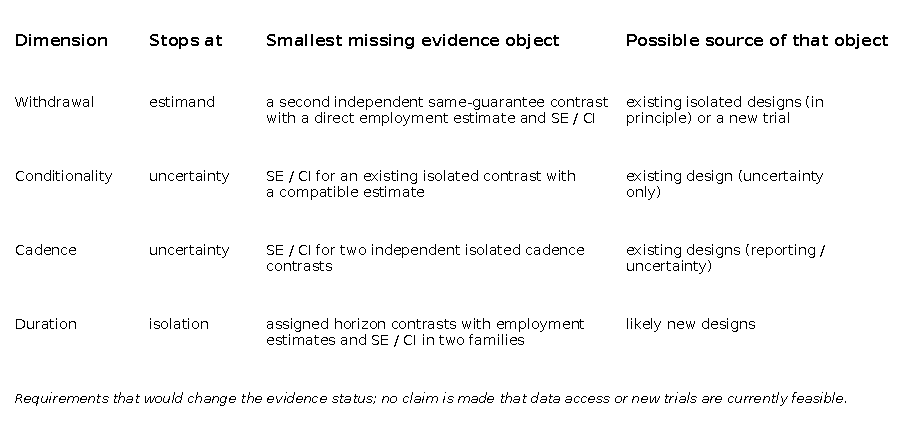
\includegraphics[width=\textwidth]{fig5_status_changing_evidence.pdf}
\caption{Status-changing evidence by dimension (former main Figure~5). For each dimension, the binding support stage and the evidence object whose availability would change its feasibility status. The figure shows no effect sizes, signs or statistical significance, and it makes no claim about whether any route is accessible.}
\label{fig:s1}
\end{figure}

\end{document}
